\section{Background}

% % Brief "what is this?" section to explain structure of background
% If we are to visualize accessibility,
% a general understanding of research in both accessibility and cartography is necessary.
% After briefly presenting both fields,
% I will relate the two together
% providing a more focused synthesis of the aspects most relevant to this thesis.

% \begin{itemize}
% 	\item Define terms more in depth (cartography, map, accessibility...)
% 	\item Small history recap of the relevant advances in the field of cartography
% 	\item Cartographic interaction theory
% 	\item Web mapping advances and technologies
% 	\item Interactive accessibility presentations and other relevant maps: go over some previous implementations and solutions.
% \end{itemize}

% Cartography - How we got to where we are now, what this means for the topic
\subsection{Maps, cartography and cartographic interaction}

\subsubsection{Defining \enquote{map}}
While the meaning of the word \textit{map} seems obvious,
defining it has been anything but simple for cartographers.
In a review of various historical writings \textcite{and1996}
found 321 unique definitions for the word.
Most of these definitions shared the premise that
maps are representations of the surface of the earth,
but, other than that, not many similarities were found.
More recent efforts in defining the word range
from lengthy attempts at precise delineation
(for example \textcite{ica2003})
to much shorter definitions (for example \textcite{kra2017}).
Currently, the \presentacr{ica},
the authoritative international body for cartography,
defines map as \enquote{an abstract visual representation of the geo-environment}
\parencite{ica2019}.

% What map for real?
Even though quite concise,
\acrshort{ica}'s definition has received its fair share of critique as well.
For example, \textcite{lap2021} note that
a map can be a concrete object or have concrete qualities
instead of being strictly abstract,
and be perceived with senses other than vision.
The word \enquote{geo-environment} is problematic too.
It would limit maps to depicting only earth
-- an issue found in many map definitions \parencite{tyn2014} --
as well as introduce possible confusion with themes such as
environmental sustainability \parencite{lap2021}.
As a response, \textcite{lap2021} suggest that,
instead of a given environment or a type of map,
\textit{spatial relationships} should be the starting point of defining what a map is.
Thus, \citeauthor{lap2021} arrive at the following definition:
\enquote{a map is a generalized representation of spatial relationships}.
A few years earlier, \textcite{tyn2014} shared much of the same sentiments,
defining a map as \enquote{a graphic representation that shows spatial relationships}.
While in her definition \citeauthor{tyn2014} specifies maps as something graphic,
both authors are in agreement that maps are representations,
and that representing spatial relationships is what makes a representation a map.

% What does "representation" mean?
% \textcite{mac2004}, along the same lines, goes as far as to say

\subsubsection{Cartography as a science}
% What cartography?
% This paragraph could move to the definition section above
It is known that
maps have been made and used in human communities for thousands of years
(for example \textcite{hsu1993, sch2014}).
However, cartography,
not as in the practice of mapmaking but as in an established science,
is much younger.
In fact, \textcite{woo2003, kai2020, cra2018} argue that
the discipline of cartography dates back only to the early 1900s,
since that is when a scientific body of theory on maps started to form.
Before that, it was mainly the mathematical theory on map projections
and the production of topographical maps
that were associated with cartography \parencite{kai2020}.
In the time that cartography has been considered its own science,
change has been a constant in the discourse within the discipline \parencite{mac2004} --
% the discipline has reinvented itself many times.
cartography is as dynamic as the topics that people map,
or the methods they use to map said topics \parencite{tyn1992, tyn2014}.
Consequently,
the term cartography has been difficult to define \parencite{kry1995},
and even if a definition is agreed upon,
it should be considered a product of the time period
in which it was envisioned \parencite{tyn1992, and1996}.
Currently, \acrshort{ica} defines cartography as
\enquote{the science, art, and technology of making and using maps}.
\parencite{ica2019}.

To better understand the discipline of cartography,
it is essential to acknowledge
the field's multidisciplinary, dynamic and multi-paradigmatic nature.
Often, methods of other disciplines are used in cartography,
and, perhaps even more often,
maps and cartography act as tools for other disciplines \parencite{kai2020}.
What these overlapping disciplines are, changes as the field evolves
and the paradigms within cartography shift
\parencite{kai2020, mac2004}.
% TODO list relevant fields -> tell that their relevance changes through paradigm shifts
% Maps and cartography are tools for all spatial sciences
% Mathematics
% Computer science
% Psychology
% Social sciences
At first, as stated earlier,
it was mathematics that was the science most relevant to mapmaking and cartography.
Representing the curved surface of earth  %, a geoid in shape,
on a surface of a different shape, often a plane when maps are concerned,
requires a mathematical transformation \parencite{tyn1992}.
In the context of cartography, this transformation is called a map projection.
The effects the projection has on a map vary by
the properties of the specific transformation used and the scale of the map,
but are always present as distortions introduced to the map \parencite{tyn1992}.
This has direct influence on how a map works, both in the sense of
its visual composition and
how the map reader understands the map \parencite{ker2018}.

% For example producing general purpose maps using a projection intended for navigation purposes.

% 1950
A map only gains meaning when it is read \parencite{gri2017}.
The process of reading a map comprises, for example,
perceiving, judging and reasoning,
often problem-solving and learning too \parencite{mon2002}.
All these are cognitive processes \parencite{apacog},
so it is clear how the field of psychology is fundamentally tied with cartography.
Initially, the link between cartography and psychology
was motivated by a shift in the discourse within cartography:
Like many disciplines post World War II,
cartography strived for credibility through empirical science.
Instead of objects of art and graphic design,
maps should be considered scientifically dissectable representations
with the primary function of conveying information \parencite{rob1952}.
Called functional map design,
this movement in cartography employed scientific methods,
especially those of psychology,
to find objectively provable rules
for producing as functional as possible maps \parencite{mon2002}.
For example,
research to optimize cartographic methods, such as symbology or labelling,
was carried out by utilizing empirical studies on human perception \parencite{mac2004}.

% ken2018, Boa2017, fai2021
In addition to studying and improving the function of maps,
functional map design had an essential role in conceptualizing \textit{how} maps function.
Already present in the work of \textcite{rob1952},
the initial concept of map function was strongly linked to graphical communication.
Drawing inspiration from studies in psychology and information sciences,
this discourse was only strengthened in the following decades
in what can be referred to as the paradigm of cartographic communication \parencite{fai2021}.
The premise of cartographic communication is
that a map is a component in a communication system,
in which its purpose is to transport knowledge to the map reader
\parencite{Boa2017}.
Many varyingly intricate models of cartographic communication exist,
but the main principles are that \parencite{ken2018}:
\begin{enumerate}
	\item The knowledge a map reader gains from reading a map is that of the mapper's,
	just transferred through cartographic communication.
	\item The main purpose of the cartographic method is
	to minimize the loss of information in that transfer.
\end{enumerate}

% With the latter half of the twentieth century,
% the relevance of computer science
While the concept of cartographic communication was
a widely used premise in cartographic inquiry \parencite{ken2018},
the discipline soon evolved into other directions.
The latter half of the twentieth century saw many developments in computer science
that, in turn, enabled notable advances in spatial computing and cartography:
for example, computer-stored spatial data,
computer-assisted spatial modelling, and, eventually,
maps presented as computer graphics \parencite{kai2020}.
As a result, the function of maps widened
and the paradigm of cartographic communication was found quite limiting.
For example, if the acts of making and reading maps were strictly equivalent to
encoding and decoding messages,
no new knowledge would be constructed by the map reader in reading a map \parencite{mac2004}.
As maps started to increasingly be used
as exploratory and analytical devices,
this was not necessarily the most fitting way of thinking of them.
Often the mapmaker and reader were the same person,
and the purpose of the map was not strictly to communicate
but also to facilitate analytical thinking
-- in other words produce new knowledge \parencite{tob2000, ant1999, kry1995}.
With its roots in analytical cartography \parencite{tob1976},
this concept of map usage first gained significant traction known as
cartographic visualization \parencite{ant1999},
a subset of the wider trend of scientific visualization
enabled by computer graphics \parencite{nie1997}.
Currently, this paradigm is best known in the form of geovisual analytics
which is also considered a science in its own right \parencite{rob2017b}.

\enquote{The map is never neutral} \parencite[p.~15]{har1989}.
\citeauthor{har1989}'s view on the nature of maps set in motion
a notable shift in the cartographic discourse
that became known as critical cartography \parencite{cra2018}.
At the core of critical cartography is the notion that
maps can never be objective sources of truth --
rather, they are socially constructed instruments of power
that ultimately reflect the ideologies of their makers \parencite{har1989}.
This sociocultural critique of maps and mapmaking
heavily contrasted the earlier paradigms in cartography.
Previously, the often implicitly authoritative map was
assumed to be capable of neutral knowledge transfer,
and the methods by which it was studied were in many cases positivist in nature
\parencite{cra2018, fai2021}.

% Multi-paradigm present day
As one main takeaway it should be recognized that
while I presented the above paragraphs quite linearly,
the multiple paradigms and disciplines relevant to cartography co-exist.
For example,
the role of mathematics is always essential to cartography --
be it the study of map projections \parencite{ker2018},
or the development of the mathematical methods
by which phenomena are represented on a map
\parencite{fra2000}.
Cartographic studies focusing on the empirical study of human perception
have continued in the context of optimizing cartographic methods (for example \parencite{yan2023})
as well as been applied to new types of maps (for example \textcite{col2009}).
The cartographic communication model still acts as a basis
for many conceptualizations of map function and, as such,
is highly relevant to cartographic research \parencite{ken2018}.
The paradigm of geovisual analytics is thriving,
largely enabled and amplified by the advances of geographic information systems (\acrshort{gis})
and other platforms that advance the analytical and explorative power of maps
\parencite{rot2013a, kra2017, lv2017}.
Critical cartography has lead to the acknowledgement of the power of maps
\parencite{cra2018, pic1995},
and to qualitative and mixed-methods approaches to studying and crafting them
\parencite{suc2000, cop2009}.

% Draws heavily from the paradigm of graphical communication,  % useless line?
% \textcite{bal1966} propose a term, "graphicacy",
% to relate the importance of graphical communication to literacy, articulacy and numeracy.
% Among the pioneers of this way of thinking about maps was \textcite{kol1969},
% who explicitly regarded maps as communication systems.

% Critique of positivism, parallel to psychophysics
% As the communication model evolved and eventually gained competition,


% Fields relevant in the sense of development of the tools of cartography,
% for example computer science \parencite{mon1985}


% \parencite{kai2020}


% % 1970
% % Cartography as graphic communication.
% The second was the change in how a map is thought to work.

% However, there have been numerous objections to the paradigm of Cartography as a form of communication.
% Firstly, there is the issue of communication versus function:
% A mapmaker might not have an intent to communicate any particular message to begin with.

% Also, implicit vs explicit:
% the message the map reader extracts from a map might differ from the one intended, or


% % Moving on from these
% Art and science \parencite{mac2004, tyn1992}  % compare these

% 1990
% - More interlinked with GIS
% - critical / qualitative GIS too

% 2010-the present -> interactive
% The change in cartography
% Rise of open source \textcite{pet2015}


% Different types of maps

% TODO
% For most of humanitys history maps have been a tool to describe the physical world,
% used for navigation and comprehending places etc
% Nowadays data visualization
% Presenting the world (locations) vs presenting data linked to locations (thematic mapping, \parencite{tyn1992})

\subsubsection{Defining \enquote{cartographic interaction} and \enquote{interactive map}}
\label{defining cartographic interaction and interactive map}

% What is interactive cartogra
So far I've referred to any persons viewing maps mostly as map readers.
\textit{Cartographic interaction} refers to a process
in which the map reader interacts with the map,
manipulating it and thus becoming an active map user, even a mapmaker,
instead of a passive map reader \parencite{rot2017}.
Originally, the concept of interaction is rooted in social theory,
where it comprises the actions and reactions in
two-way communication between humans \parencite{ken1996}.
However, with the advance of computer technology,
interaction theories have been increasingly applied and developed
in the context of dialogue between humans and computers \parencite{qui2008}.
This is known as \emphasizeacr{hci}.
In addition to the process, \acrshort{hci} is a field of research examining
the function of interactive User Interfaces (\acrshort{ui})
and \presentacr{ux}
in the context of dialogue between computers and humans \parencite{car1997, hor2017}.
Interactivity, then, can be
a property, a perception, or an experience \parencite{lan2023},
and, depending on how it is conceptualized,
it can be modelled and studied in a multitude of ways \parencite{smu2009}.
Additionally, it must be noted that interaction and interactivity are factors
that depend not only on the technologies and
contexts of dialogue, but also on people’s perceptions and capabilities
\parencite{kio2002, duc2018}.

At the most general level of definition,
cartographic interaction can refer to
any type and level of interaction with any kind of map \parencite{pet1998}.
In fact, \citeauthor{pet1998} goes as far as to argue
that the static map of the modern times is the exception:
Interaction, for example collaborative mapmaking
as a communicative aid in social contexts
(figure \ref{fig:paper interactive map}),
has been the norm of making and understanding maps
before they were transformed into static artefacts,
be it printed or digital images.
Currently, cartographic interaction and interactive maps
are most often connected to digital applications
where a map either is \textit{the} interface,
or a significant part of the interface of an application
(figure \ref{fig:digital interactive map}) \parencite{mei2019}.
Regardless of the medium of the map,
the key concept that is agreed upon is that cartographic interaction necessitates
a map that can be manipulated by the map user,
blending map use and mapmaking at the conceptual level \parencite{rot2015}.
When contextualized within the topics and paradigms of cartographic research,
studies on cartographic interaction can be understood as
mainly focusing on the processes of mapmaking and interaction
instead of map use and representation \parencite{rot2013b}.
While these distinctions are by no means absolute,
they can help provide an outline of interactive cartography in
relation to other topics of research in cartography (figure \ref{fig:cartography topics}).

\begin{figure}[H]
	\centering
	\includegraphics[width=0.75\textwidth]{visual/figures/photos/paper_interactive_map.png}
	\caption{
		An interactive paper map about travel experience in urban space.
		Constructed in a workshop setting,
		it enables cartographic interaction
		through manipulation by post-it-notes and annotations.
		Here the process of mapmaking is also a social one,
		as it both facilitates and is facilitated by
		human to human interaction about the mapped topics.
		Photo by Christoph Fink.
	}
	\label{fig:paper interactive map}
\end{figure}

\begin{figure}[H]
	\centering
	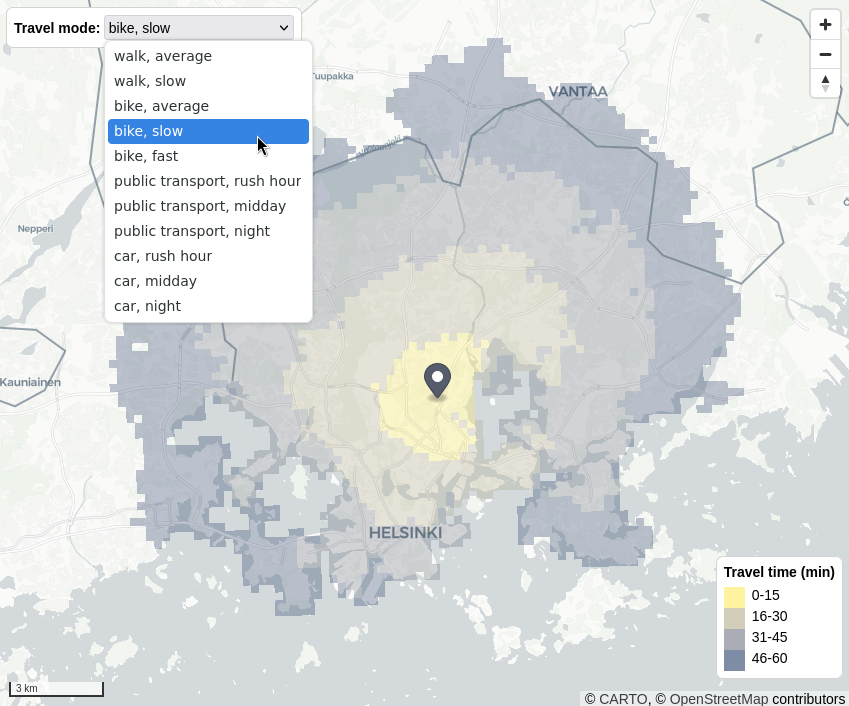
\includegraphics[width=0.9\textwidth]{visual/figures/screenshots/digital_interactive_map.png}
	\caption{
		A screenshot of a digital interactive map about travel times.
		In digital interactive maps
		cartographic interaction happens through a graphical UI,
		where the map can be manipulated by the user.
		Here the user can, for example,
		change the extent of the map by panning and zooming,
		and change the mapped data by selecting different options in a drop-down menu.
	}
	\label{fig:digital interactive map}
\end{figure}

\begin{figure}[H]
	\centering
	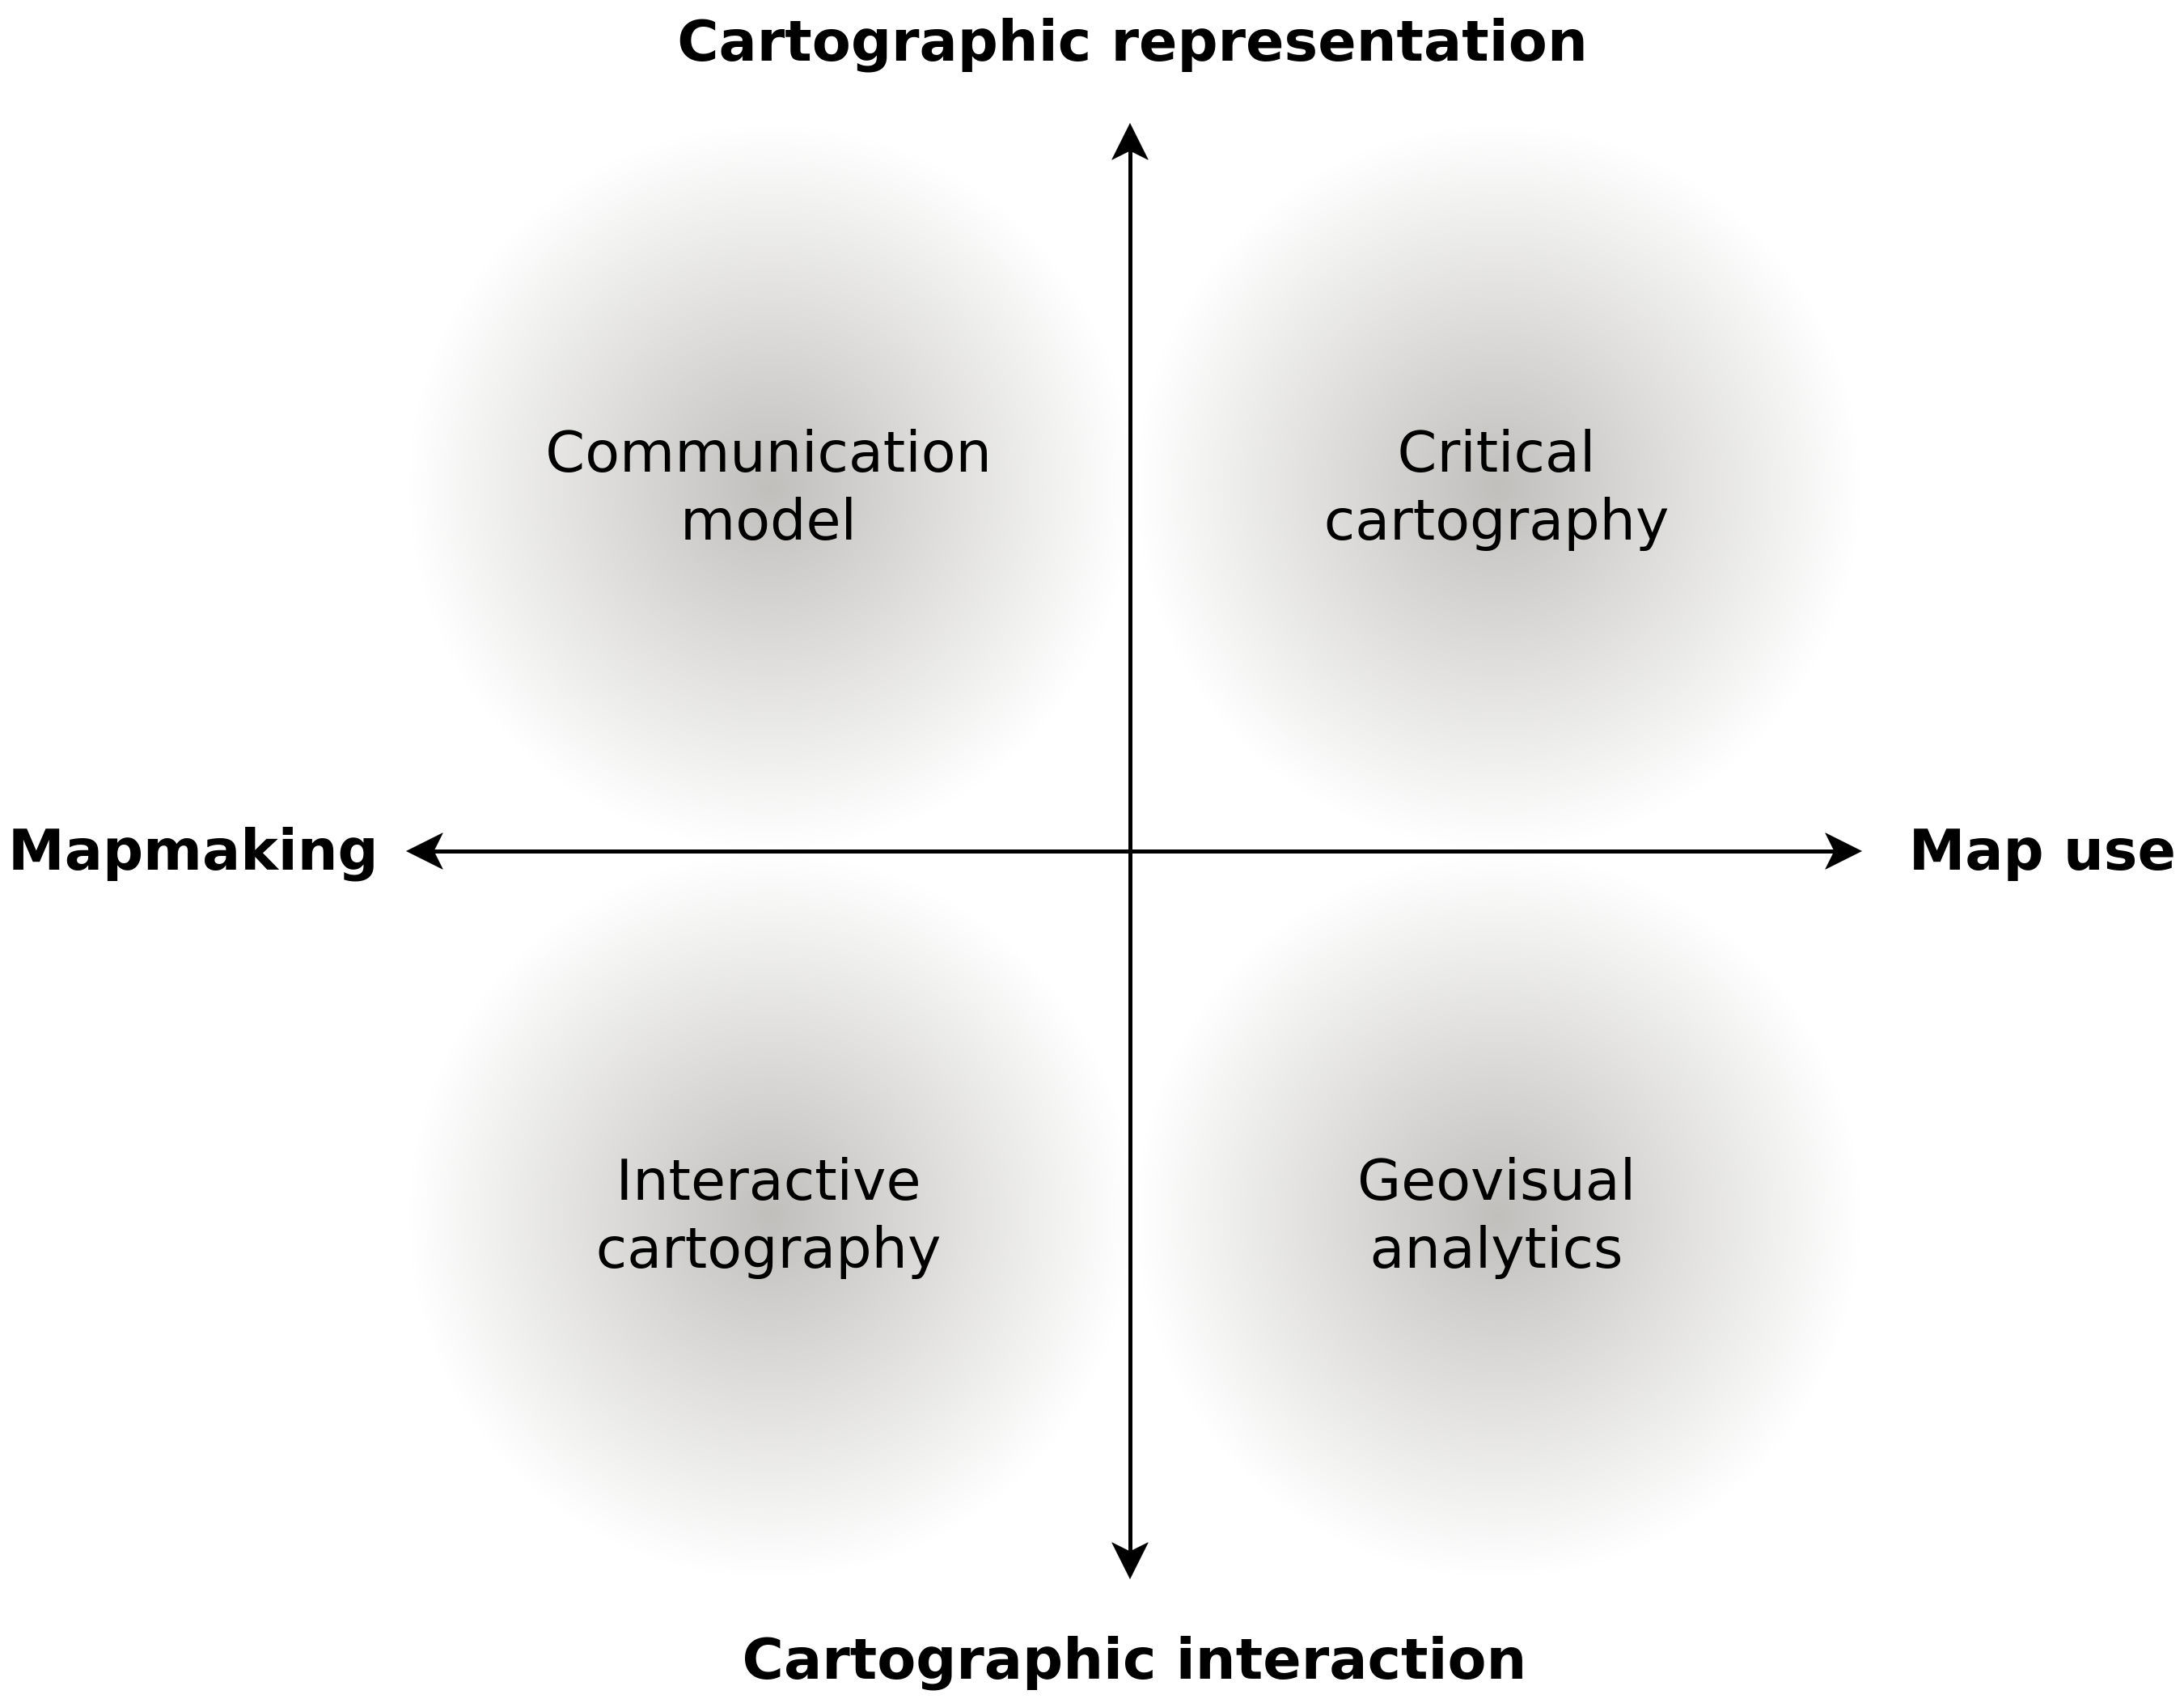
\includegraphics[width=\diagramwidth]{visual/figures/diagrams/cartography_topics.png}
	\caption{
		Interactive cartography as a topic of research
		in relation to other notable topics within cartography.
		The circles representing topics are fuzzy to imply that,
		instead of clear separation,
		different topics and areas of research blend into each other.
		Adapted from \textcite{rot2013b}.
	}
	\label{fig:cartography topics}
\end{figure}


In this thesis I approach cartographic interaction as
two-way communication between a map and a map user,
but limit it to digital maps and \acrshort{hci}.
As defined by \textcite[p.~14]{rot2011},
\enquote{Cartographic interaction is the dialogue between a human and a map
mediated through a computing device}.
The dialogue, or two-way communication, is a crucial aspect of this definition
as it makes explicit that in addition to the map user manipulating the map,
the map also affects the user:
The map user's interactions result in changes in the map,
and those changes, through the map user perceiving, interpreting and evaluating them,
can alter the map users goals and intentions
in further manipulating the map (figure \ref{fig:map interaction}) \parencite{rot2012}.
This conceptualization of cartographic interaction
is based on \posesscite{nor1988}
stages of action model that,
in contrast to many other theories on human-object-interaction,
places agency to both the human and the object.
Another aspect worth noting in \posesscite{rot2011} definition
is the notion of interactive maps as digital applications.
This is a relevant approach considering
that the mediums in which people interact with maps today
are predominantly and increasingly digital \parencite{mei2019}.
Digital environments also enable more ways to interact with maps
and to construct interactive map presentations \parencite{rot2013b, mei2019}.
Considering the aforementioned definition of cartographic interaction,
I deduce that, in the context of this study,
an \textit{interactive map} is a digital one,
and for it to be considered interactive it has to
facilitate a dialogue by enabling and adapting to manipulation by the map user.

\begin{figure}[H]
	\centering
	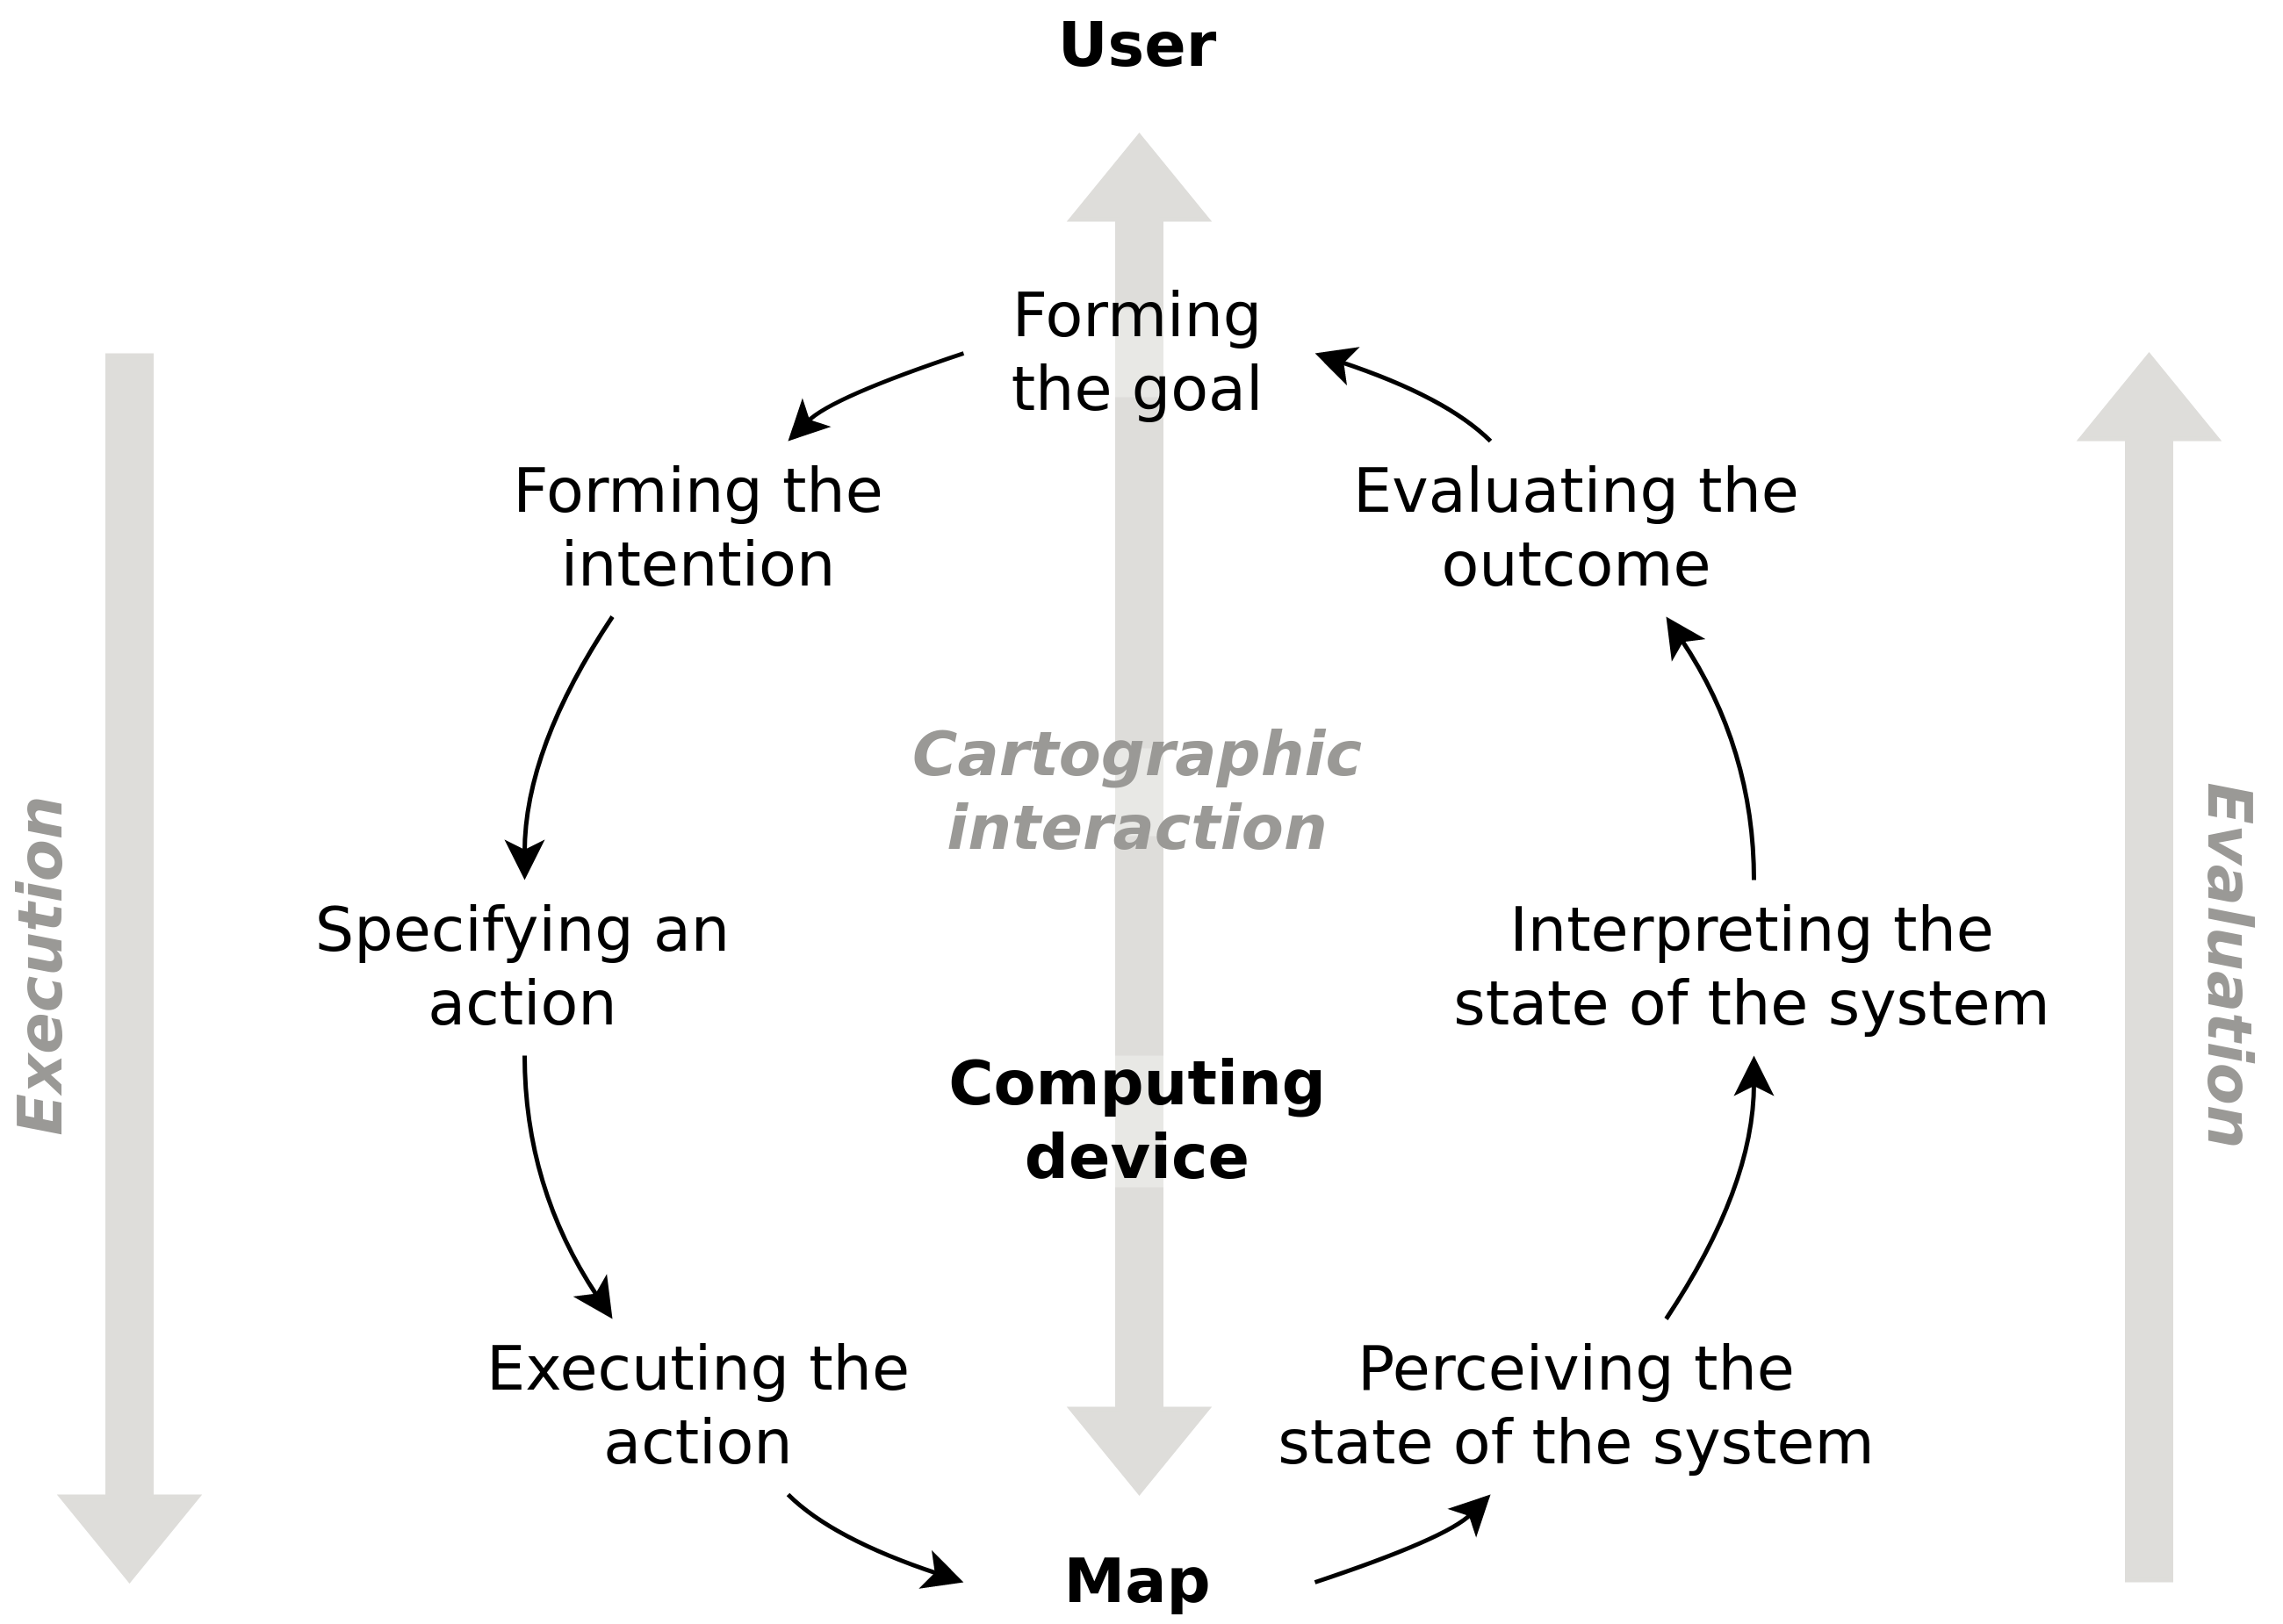
\includegraphics[width=\diagramwidth]{visual/figures/diagrams/map_interaction.png}
	\caption{
		The process of cartographic interaction.
		\posesscite{nor1988} stages of action model,
		a foundation of the concept of human-object-interaction as dialogue,
		is here applied to cartographic interaction.
		Adapted from \textcite{rot2012}.
	}
	\label{fig:map interaction}
\end{figure}


\subsubsection{Perspectives and disciplines relevant to interactive cartography}

Cartographic interaction, as defined above, has three components:
the human as the user, the map as the interface,
and the computing device as the technology that enables the interaction.
% Arguably, there is a fourth component too: the dialogue.  % TODO
While cartographic interaction as a concept should be approached as
the sum of its parts \parencite{rot2013b},
studies on cartographic interaction can take on perspectives
that emphasize given subsets of these components.
For example, \textcite{col2009} approach the topic from a user-centric perspective,
\textcite{rot2013a} has an interface-centric focus in
taxonomizing various interaction primitives in map interfaces,
and \textcite{oym2021} develop a technological method and an implementation
for producing interactive maps.
I should also stress that I do not wish to imply that these studies
only recognize the singular components of cartographic interaction
I've associated with them here.
Rather, they approach the topic from a perspective relevant to their respective goals,
but they do account for the other components as well.

% HCI
The components of cartographic interaction widen the scope of cartography,
also further motivating and calling for
multidisciplinary approaches in the field \parencite{rot2013b}.
As maps become interfaces,
\acrshort{ui} and \acrshort{ux} research and design becomes
part of the process of mapmaking \parencite{rot2015}.
Thus, the research, theories and methods in \acrshort{hci}
and \presentacr{ue} have been notable influences
digital interactivity has introduced to the discipline of cartography \parencite{rot2017}.
These can for example be new empirical approaches such as
data acquisition through system or application level recording and storage of
user interactions with digital map interfaces \parencite{oom2015}.
Research on the different technological aspects and modes of \acrshort{hci}
has also been carried out in cartographic contexts,
for example by evaluating different input devices and methods
used in interacting with web map applications \parencite{wu2011}.

% UE
The usability of interactive map presentations has been studied with
usability metrics often employed in \acrshort{ue} research more widely.
These include but are not limited to
user satisfaction (how content users are with an interface having used it),
efficiency (how quickly users complete tasks with an interface)
and effectiveness (how successful users are at completing tasks with an interface)
\parencite{col2009}.
When considering usability, it should also be noted that interactive maps,
often relying solely on computer graphics for all aspects of their interface,
can introduce notable usability issues
to people without the capabilities to interact with such interfaces \parencite{duc2018}.
These issues can stem from the more general limitations of accessing digital applications --
for example lack of technical knowledge or unfamiliarity with a specific interface \parencite{kul2019} --
but are especially severe when it comes to visual impairments,
potentially leading to complete exclusion from accessing an interface \parencite{duc2018}.
Still, it has been shown that cartographic interaction can be made inclusive:
By introducing methods such as tactile and audio interaction,
interactive maps have been observed to be more efficient and satisfactory interfaces
for visually impaired users when compared to tactile static maps \parencite{bro2015}.
In general, as informed by \acrshort{ue},
the need for user perspective in studies on cartographic interaction has been recognized,
and user-centred and inclusive design practices are considered beneficial to map interface design
\parencite{niv2007, rot2017, duc2018}.

Even though briefly mentioned earlier,
geovisual analytics should also be highlighted as
a discipline that is especially relevant to interactive cartography.
Defined as \enquote{the science of analytical reasoning with
spatial information as facilitated by interactive visual interfaces}
\parencite{rob2017b},
it is clear that the field is largely enabled by
cartographic interaction.
In contrast to research in \acrshort{hci} and \acrshort{ue} --
both fields that are focused mainly on interfaces as primary objects of study
\parencite{mol2023, car1997} --
studies in geovisual analytics are more concerned with
how map interfaces enable and support analytical processes \parencite{rob2017b, and2010}.
An analytical process in this context consists of, for example,
assessing data and extracting insight from it (exploration),
studying and contrasting different insights (analysis),
disseminating results (presentation),
and integrating and reasoning about different insights and results (synthesis) \parencite{mac2017, dib1990}.
From the perspective of cartography and especially cartographic interaction,
this type of approach relates the map interface to many different stages and types of reasoning.
Thus, an interactive map can, often simultaneously, be
an interface to a multitude of analytical methods,
an analytical method in and of itself,
a means to satisfy many different analytical goals and needs,
and a platform for various methods and modes of interaction \parencite{rot2013b, rot2015}.

In the cartographic context,
the role of interactivity has often been considered most essential to
exploration and analysis \parencite{eds2008}.
At these stages of the analytical process,
the creation of numerous and / or highly interactive maps
enables rapidly gaining and assessing insights,
while the stages of synthesis and presentation
have classically been seen to employ fewer,
more static, presentations
(figure \ref{fig:analytical process interaction}) \parencite{dib1990}.
While interactive maps are still often connected to exploration,
their potential in presenting known insights (for example \textcite{ecc2008}),
as opposed to only revealing new ones through exploration,
has been recognized and growingly applied \parencite{fis2021}.
This proliferation of cartographic interaction is also visible in the state of mapmaking:
in practice, interactivity is being increasingly utilized
in most contexts where maps are present \parencite{fis2021, mei2019, rot2015}.

\begin{figure}[H]
	\centering
	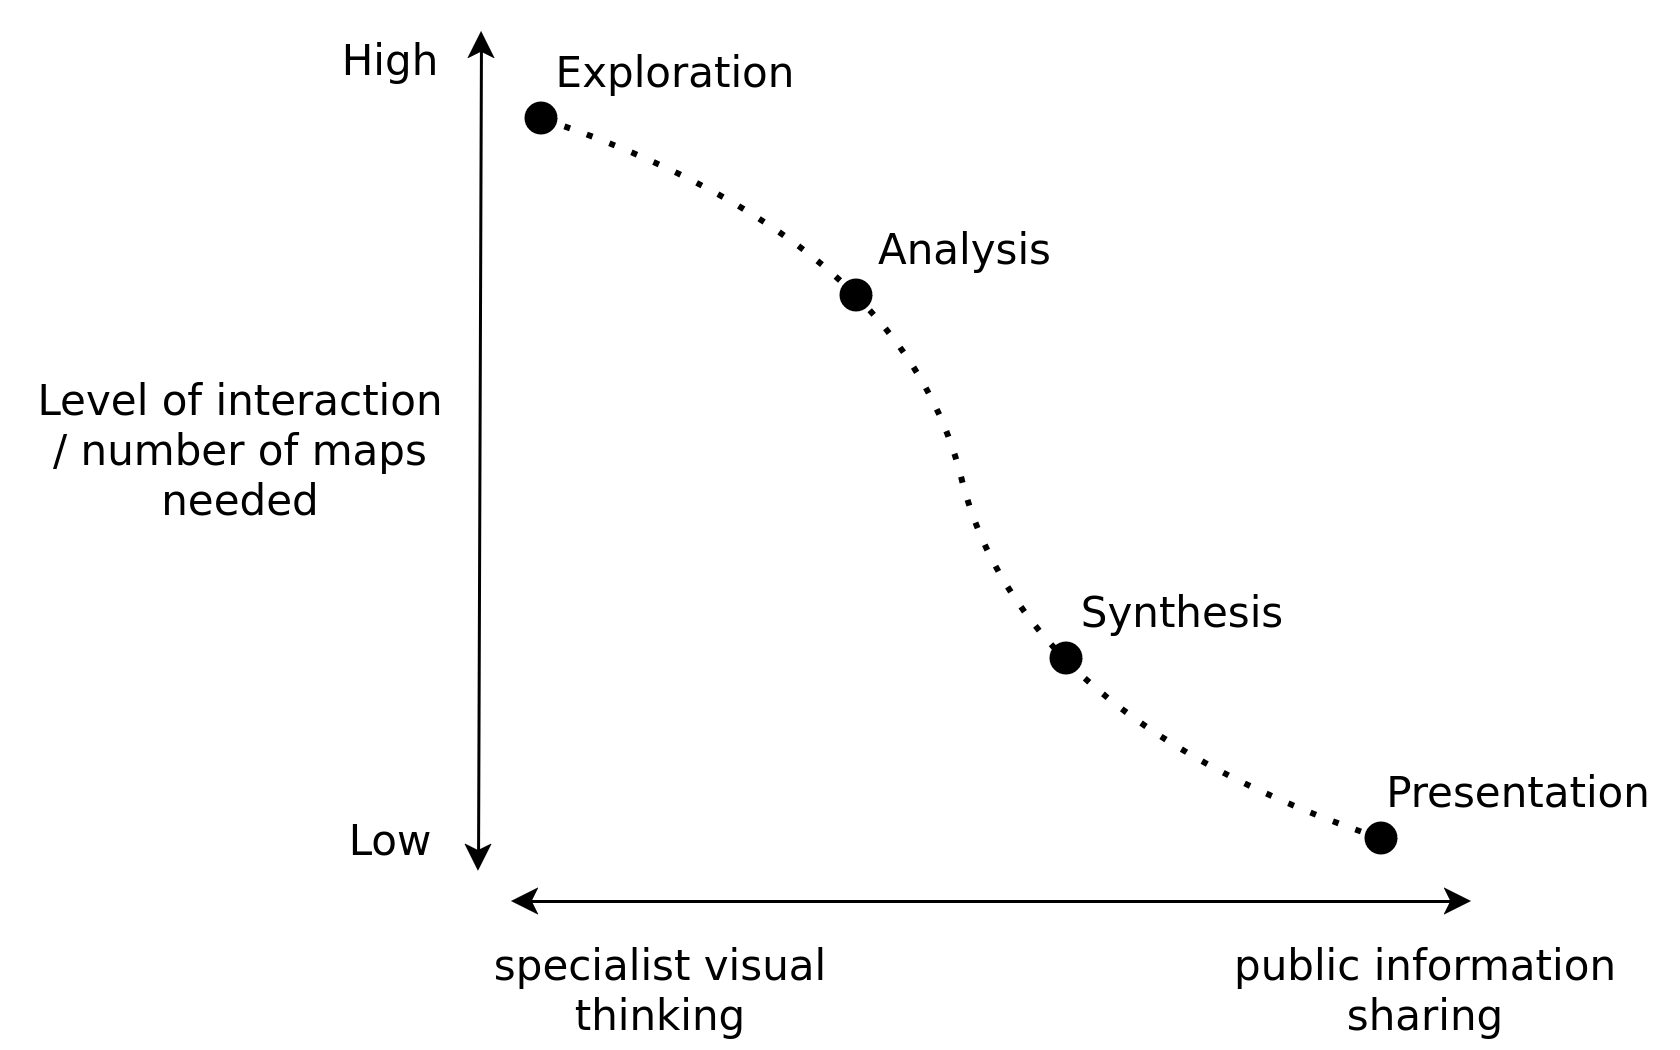
\includegraphics[width=\diagramwidth]{visual/figures/diagrams/swoopy.png}
	\caption{
		The need for interactivity at various stages of an analytical process.
		Considering the developments in cartography since 1990,
		the slope might be slightly gentler today.
		Adapted from \textcite{dib1990} with minor changes in wording based on
		\textcite{rot2015, mac1997}.
	}
	\label{fig:analytical process interaction}
\end{figure}


\subsubsection{Deconstructing the map interface}

What exactly an interactive map is,
or what kind of interaction exchanges a user can carry out with the map,
varies greatly.  % depending on what the purpose of the map is.
As is clear based on the above,
the applications of cartographic interaction are immensely diverse,
and so are the different types of map interfaces.
Thus, conceptualizing the many forms of
interactive maps and the interactions they enable
at a detailed level is no simple task.
Soon to be 20 years ago,
\textcite{tho2005} considered the comprehensive
identification, characterization and compilation
of the various types of interactions in visual analytics a
\enquote{grand challenge of interaction}:
a prerequisite for the effective design and utilization of
interactivity in analytical processes.
Since then, and also predating \posesscite{tho2005} work,
this research topic has been widely explored in many relevant fields.
In an extensive literature review \textcite{rot2012}
provides a synthesis of tens of studies
that propose varying taxonomies of interaction,
especially in the context of interactive maps.
As a high-level output of the study, \citeauthor{rot2012}
classifies interaction taxonomies into three categories:
Objective-based, operator-based and operand-based.
Objective-based taxonomies categorize interactions based on
the objective behind the interaction,
for example to select, explore or encode \parencite{yi2007},
while operator-based taxonomies act at the level of operations such as
zooming, panning or altering representation types \parencite{eds2008}.
Operand-based taxonomies classify interactions based on what is operated upon.
This could be, for example, data, the representation of said data,
or the interface itself \parencite{cra2002}.

Building upon these insights,
\textcite{rot2013a} proposed a taxonomy of interaction in a follow-up study.
While, again, multiple such efforts exist,
\citeauthor{rot2013a}'s taxonomy is perhaps the most relevant in this case:
It is constructed from the perspective of cartographic interaction,
and informed not only by a review of other taxonomies \parencite{rot2012}
but also by empiric studies with experts in the field of interactive cartography
\parencite{rot2013a}.
This taxonomy is based on \textit{interaction primitives} --
basic units of interaction that, when combined,
make up complete interaction exchanges between a map and a map user.
These interaction primitives are grouped into 4 dimensions:
\textit{objectives}, \textit{operators} and \textit{operands}, as already described above,
with the addition of user \textit{goals} as a broader context of
an interaction exchange \parencite{rot2013a}.
As another added level of detail, operator primitives are split into primitives that
enable work and primitives that represent the work itself,
and operand primitives are split into targets that are operated
upon and levels on which the operation happens.
\enquote{Level} in this context means the scope of the operation:
either elementary (one element) or general (multiple elements) \parencite{rot2013a}.
For the complete taxonomy, see table \ref{tab:interaction primitives}.

\begin{table}[H]
	\caption{
		\posesscite{rot2013a} taxonomy of interaction primitives.
		A taxonomy such as this is required for the systematic description, study and design
		of map interfaces.
	}
	\label{tab:interaction primitives}
	\centering
	\begin{tabular}{ | L{0.15\textwidth} | L{0.75\textwidth} | }
		\hline
		\textbf{Dimension}
		& \textbf{Primitives} \\
		\hline
		\hline
		Goals
		& Procure, predict, prescribe \\
		\hline
		Objectives
		& Identify, compare, rank, associate, delineate \\
		\hline
		Operators
		& \tabitem Enabling operators: import, export, save, edit, annotate \\
		& \tabitem Work operators: reexpress, arrange, sequence, resymbolize,
		overlay, reproject, pan, zoom, filter, search, retrieve, calculate \\
		\hline
		Operands
		& \tabitem Target operands: space-alone, attributes-in-space, space-in-time \\
		& \tabitem Level operands: elementary, general \\
		\hline
	\end{tabular}
\end{table}


In general, interaction primitives
address the \textit{what} in an interaction exchange:
for example, what the goal is, what the operation is, or what is operated upon.
A wider theoretical framework of interaction, such as the one presented in
section \ref{defining cartographic interaction and interactive map},
is necessary to understanding \textit{how} interaction works as a whole.
What I have not yet covered in detail is
\textit{how} interactions are carried out at the level of the interface, or,
in other words, how the interactivity is provided to the user.
In the context of \acrshort{hci},
the ways in which a user can interact with a system are referred to as
\textit{interaction styles} \parencite{shn1995}
(sometimes also \textit{interface styles} \parencite{how1996}).
These are conventionally categorized into 4 main styles:
\textit{command language},
\textit{form fill-in},
\textit{menu selection} and
\textit{direct manipulation}
\parencite{soe2015}.
Additions exist, for example \textit{natural language},
often employed in audio-based interfaces \parencite{duc2018}.
Most of the aforementioned interaction styles are quite self-explanatory,
but one; direct manipulation, depends on context.
In the case of cartographic interaction,
it refers most often to direct interactions with the map \parencite{rot2012}.
A common example would be a case where the \textit{pan} operator primitive
is executed by dragging the map with a pointing device.

When considering a map interface,
it should be noted that most operator primitives
can be exposed to the user using multiple interaction styles.
For example, the previously mentioned \textit{pan} operator could just as well
be executed with a command language, a form fill-in, or a menu selection.
What interaction style is best suited for a given operator is a question
of \acrshort{ui} and \acrshort{ux} design,
and depends heavily on the specific operator as well as
the users and the use case of the map interface \parencite{rot2015}.
This further exemplifies the diversity of interactive maps,
as interaction style adds yet another dimension to conceptualizing the
function and form of a map interface.
When assessing the interaction styles in a map interface,
one aspect that is often considered in interactive cartography
is the amount of direct map manipulation in relation to other interaction styles.
If direct map manipulation is just part of
the interaction styles provided by an interface,
the interface might be called
a \textit{map-based system} or a \textit{map-based interface}
instead of, for example,
an \textit{interactive map} or a \textit{map-interface} \parencite{rot2013b}.
A desktop \acrshort{gis} software could represent the former type of interface (figure \ref{fig:qgis}),
and a simple web map the latter (figure \ref{fig:simple web map}).

\begin{figure}[H]
	\centering
	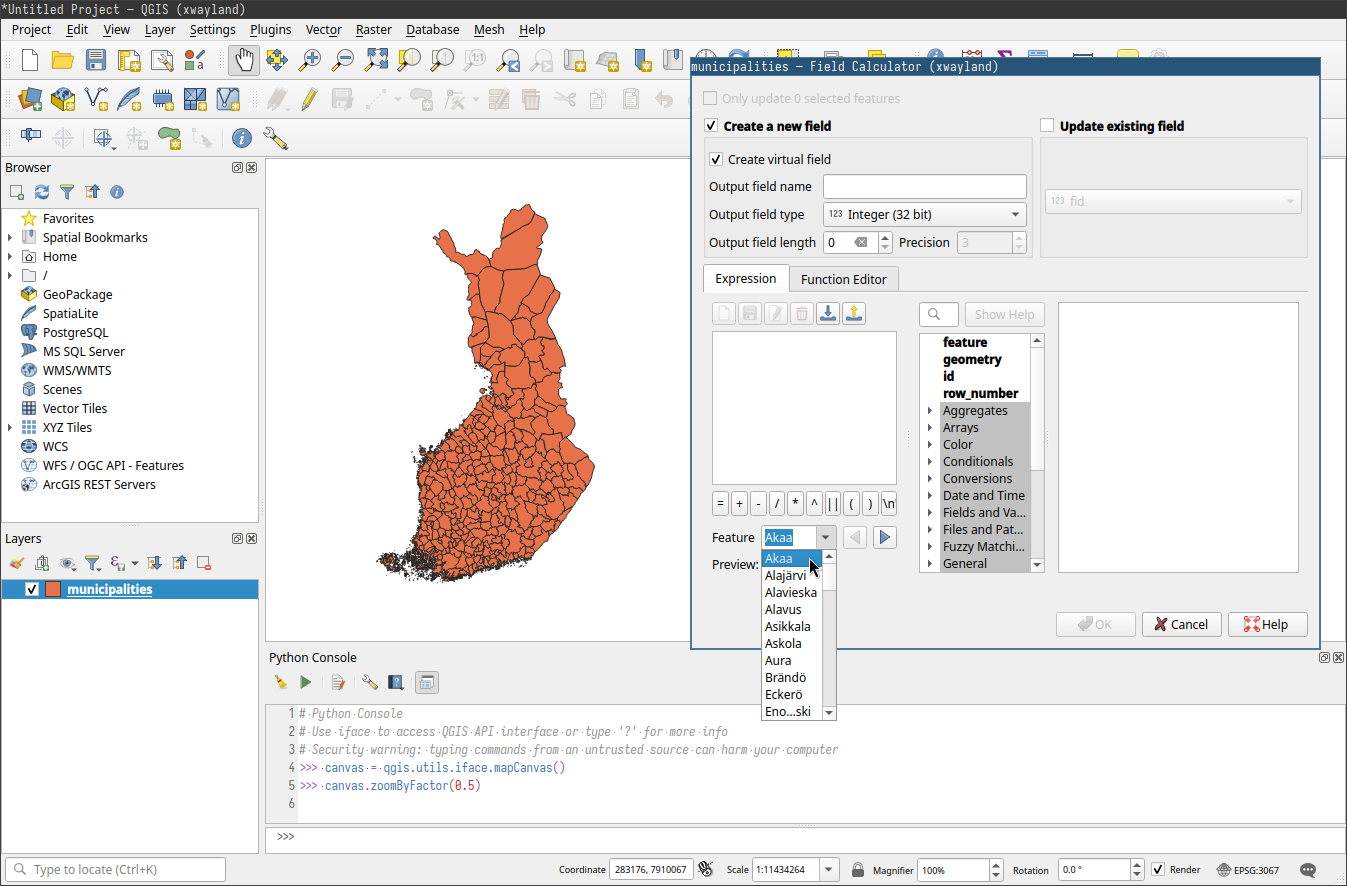
\includegraphics[width=0.9\textwidth]{visual/figures/screenshots/qgis_interface.png}
	\caption{
		The UI of the desktop GIS QGIS \parencite{qgis}.
		GIS software often supports a wide array of interaction primitives and,
		consequently, interaction styles:
		Direct manipulation, menu selection, form fill-in and command language
		can all be seen in this image.
	}
	\label{fig:qgis}
\end{figure}

\begin{figure}[H]
	\centering
	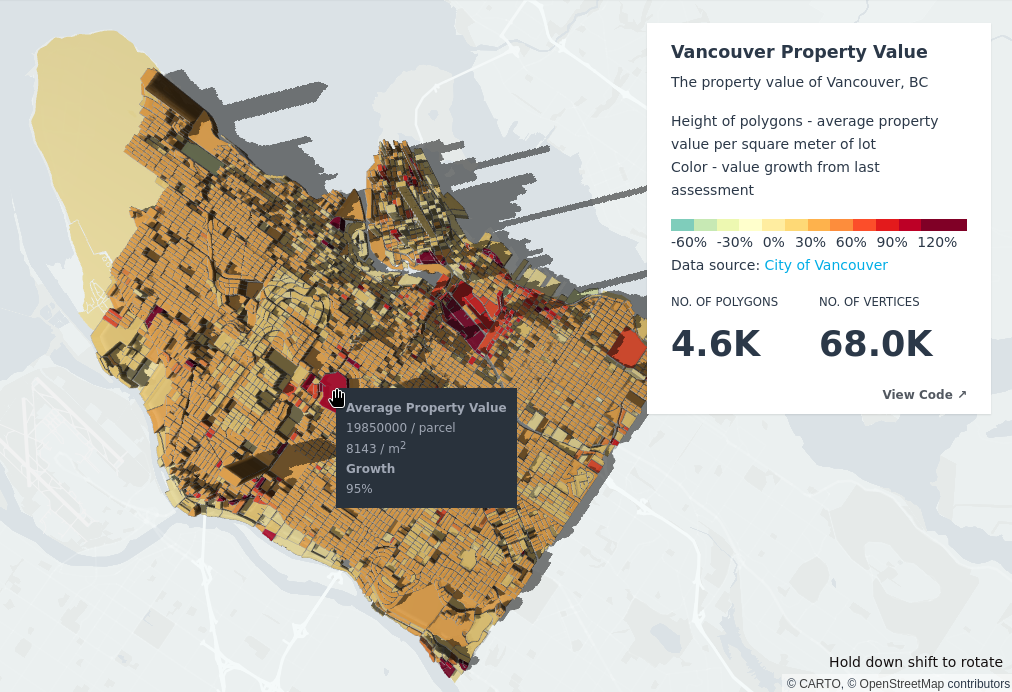
\includegraphics[width=0.9\textwidth]{visual/figures/screenshots/simple_web_map.png}
	\caption{
		An interactive web map with a single interaction style:
		direct manipulation of the map.
		Map source: \textcite{deckgl-ex}
	}
	\label{fig:simple web map}
\end{figure}

% Together with interface types the interaction primitives make up
% the building blocks necessary for understanding, analysing and designing map interfaces.


% cra2002
% Interaction with data representation (zoom, pan, symbolization)
% Interaction with the temporal dimension (animations, toggling, sorting)
% Interaction with data (exploration)
% Interaction to contextualize (multiple views, overlay)

% hee2012
% Data & view specification (visual encodings, filtering, sort)
% View manipulation (select, navigate, organize views and workspaces)
% Interacting with processes & preserving analytical provenance (record and review actions (meta-interaction))

% yi2007 (intent-based)
% 1) Select, 2) Explore, 3) Reconfigure, 4) Encode, 5) Abstract/Elaborate, 6) Filter, and 7) Connect

% rot2012 the framework

% rot2013a
% Goals: procure, predict, & prescribe
% Objectives: identify, compare, rank, associate, & delineate
% (increasing in sophistication);
% Operators: import, export, save, edit, & annotate (enabling);
% reexpress, arrange, sequence, resymbolize, overlay, reproject, pan, zoom, filter, search, retrieve, & calculate (work);
% Operands: space-alone, attributes-in-space, & space-in-time (search target);
% elementary & general (search level)



% Interactive
% In the following, the term “in-teractive” is used rather than “dynamic” to distinguish display updates evoked by the user(interaction) from display updates evoked by the system (such as animation, a form of car-tographic representation)phy - broadly  % FIXME copypasta


% \parencite{kra2017}
% The traditional ‘authoritative’ view of the map being a carefully crafted product
% by the cartographer, aimed at visually communicating a complete, mostly static database
% of known geographic facts to a user, has turned into a participatory and collaborative perspective.
% The map has moved beyond the static window to the world and become an
% interactive, mobile, dynamic and collaborative interface between a human, groups of
% people and the dynamically evolving environment



% The nature of interactive cartography
% More than a map: ui, ux
% What even is an interactive cartographer?
% A map is both the for of presentation, as well as the method of interaction
% -> a more complex map means basically a user interface -> need for UI library
% \textcite{rot2013a, rot2013b}

\subsection{Crafting interactive maps}

% The previous section provided the tools to conceptualize
% what cartographic interaction and interactive maps are.
% This section aims to add the necessary insight to
% understand how interactive maps function at a technological level


\subsubsection{Maps as digital applications}
\label{maps as digital applications}

Interactive maps were defined in
section \ref{defining cartographic interaction and interactive map}
as digital applications.
The functionalities and characteristics of an interactive map, then,
are ultimately dictated by the features and constraints of the technologies
used in implementing, presenting and interacting with the map.
This is why a technological perspective into
cartographic interaction, as enabled by a digital environment,
is an essential consideration in crafting any map interface.

% Digital environment, application
Here, I use the term \textit{digital environment} to refer to
an ecosystem of digital tools, systems and resources,
not to be confused with artificial computer-created scenes
that the word is also often associated with in cartography \parencite{kon2011}.
In general, a digital environment makes it possible to enable a map interface with
the capabilities of computer programs and other accompanying digital technologies.
From the perspective of interaction, perhaps the most notable of these
is the ability to receive input from the user and perform computations based on it,
possibly altering the state of the program.
The altered state of the program can then be communicated back to the user.
This establishes the technological premise for
the process of interaction as two-way communication.

Such an interaction exchange necessitates a computing device for executing the program,
an input device for processing user input into a digital form,
and an output device for conveying the state of the program to the user.
From a technological perspective,
the attributes of these devices are both enabling and limiting factors of
cartographic interaction as \acrshort{hci}.
The processing power of the computing device determines the speed at which
computations can be made, impacting the latency
(the delay between user input and its perceivable results)
of the system.
The input device plays a major role in what interaction styles
are usable in the map interface,
and the output device dictates how the user perceives the interface.
All these aspects directly contribute to the user's experience of interactivity.  % TODO ref

At the software level, the computer program
(often referred to as an \textit{application} in the case of user-facing software)
is ultimately what the user interacts with.
What exactly an application is, or what it does, is a complex question.
In the following, I utilize some basic concepts of software architecture
to provide a starting point to reasoning about this theme.
In the case of interactive maps,
the primary purpose of the map application is
to provide presentation and an interface,
in short, it acts as a \acrshort{ui} of
a program, or potentially a system of multiple programs.
User actions
(often called \textit{user events} in the context of software development)
result in computations as defined by the system's rules and algorithms,
\textit{business logic} in a software context.
In software architecture, such logic is a concern often separated from presentation,
which means that the computation induced by a user event might happen
in a separate component of the application,
or even be handled by an entirely different program.
Applications, especially ones concerned with mapping,
often act on data.
Storing and accessing data are distinct functionalities, and, again,
can be carried out by separate solutions
with varying levels of decoupling from presentation and business logic.
The above high-level components --
\acrshort{ui}, business logic, and data access and storage --
together with any necessary services that enable their interoperation,
can be thought to make up a given interactive system.
This approach to reasoning about the structure of a system is often connected to
\textit{layered software architecture},
but is utilized in other architectural patterns too. % TODO ref?
The main point is that
systems are often structuralized based on the functionalities of their parts,
which I here applied to help illustrate what the necessary functionalities
to enable an interactive map system might be.

% (Hardware + software + application) - the application = platform
Another key consideration of crafting map interfaces is the
\textit{computing platform} --
the execution environment a given program or system requires in order to run.
Computing platforms can be categorized to
hardware, \presentacr{os} and software level platforms.
This division can be seen in terms of abstraction layers:
A software platform runs on an \acrshort{os} platform,
and an \acrshort{os} platform runs on a hardware platform.
From the perspective of map applications,
\acrshort{os} and software platforms
are the ones to consider since they provide the capabilities,
such as advanced use of computer graphics,
needed for cartographic interaction.

The characteristics of different computing platforms
dictate much of the design and functionalities of map interfaces.
\acrshort{os} platforms are closely tied to
the devices (hardware) they operate on:
Applications developed for most mobile \acrshort{os}s
are expected to be operated mainly on relatively small touchscreens and
with potentially constrained computational capabilities,
while \presentacr{pc} \acrshort{os}s
provide an environment usually accessed with larger displays and
separate input devices, and enabled with more computational power.
Software platforms are, in practice, software that runs other software.
There are an innumerable amount of such platforms but,
to give an example, perhaps the most relevant today is the web browser.
In general, applications running on a software platform can be run wherever
the platform can be run, often meaning less dependence on particular devices.
In turn, they have much less direct access to the operating system or hardware,
potentially noticeable computational overhead introduced by running the platform
in addition to the application,
and cannot utilize features that the software platform lacks.

% The influence of technology on interactive maps and cartography.
% Also, the mapmaker is more often a software developer than a cartographer.
% How much of innovation is more of "this is cool",
% versus "this is a cartographically informed way to present something".


\subsubsection{Web maps and web technologies}

A web map is a map that is made with web technologies,
transferred via the internet,
usually accessed with a web browser,
and read and used as a web page \parencite{sac2017}.
To understand what any of this means,
it must first be acknowledged that
the web has been, and is, a rapidly changing ecosystem.
Initially intended for specialist use with the sole purpose of
sharing static documents through
interconnected computer networks (the internet) \parencite{ber1994},
it is now a platform for increasingly complex systems and applications
\parencite{mik2019}.
Consequently, what web maps are,
and what technologies they are implemented with, changes too.
In the time that the internet has existed,
the concept of a web map has gone
from a static map sent as an image, to
highly interactive map applications
and even extensive web \acrshort{gis} platforms \parencite{vee2017}.

% ber 1994, tai2017
In the context of the immense change the web as a whole has gone through,
the fundamental core concepts and technologies that the platform is built upon
have remained very constant, by comparison.
Dating back to the establishment of the platform,
\emphasizeacr{html}, \emphasizeacr{http}, and the concept of
\textit{client-server architecture}
still make up the absolutely necessary building blocks
of presenting and accessing web pages \parencite{ber1994, tai2017}.
\acrshort{html} is the markup language of the web,
primarily designed for the semantic description of documents \parencite{w3chtml},
and \acrshort{http} refers to a set of protocols for transferring information over the internet,
for example \acrshort{html} documents \parencite{ietfhttp1, ietfhttp2, ietfhttp3}.
This information is fetched by a client, from a server --
the premise of client-server architecture.
A client in this context is
a piece of software (most often a web browser) that sends \acrshort{http} requests,
receives responses that can include resources,
and potentially performs actions based on the response --
for example, renders a web page based on a received \acrshort{html} file
\parencite{sac2017}.
A server, also a piece of software,
runs on another computer or on a distributed computing platform,
\enquote{listens} for requests,
and responds to them using \acrshort{http},
potentially sending files that are stored on the computer running the sever
\parencite{sac2017}.

A web consisting only of static web pages, as described above,
is hardly reminiscent of the web today.
The progress towards an interactive web began with
dynamic website creation using server-side computing,
where a given \acrshort{html} page could be dynamically created on the server-side,
based on user input from the client \parencite{jac2019}.
This also enabled the first interactive web maps,
although interactivity in this case was still
far from responsive by modern standards \parencite{vee2017}.
The single most important factor in enabling web maps as they are today,
also resulting in the web's transformation into a software ecosystem,
was the introduction and standardization of a client-side scripting language,
\textit{JavaScript} \parencite{cho2014, vee2017}.
This is the basic requirement for \textit{client-side computing},
which is the concept that a client can
receive and execute code.
This essentially turned websites from documents
into software, often called \textit{web applications} \parencite{jac2019}.
Today, software built \enquote{for the web} refers most often to
such client-side applications -- pieces of software
that use the web browser as a computational platform \parencite{tai2017}.
Client-side technologies are also the main focus in the context of web-mapping,
since a modern web map is usually a heavily client-side application
\parencite{rot2014}.

To understand how a modern web application works,
some additional insight is still necessary.
Key factors here are the \emphasizeacr{dom} and
\emphasizeacr{ajax}.
The \acrshort{dom} defines a standardized representation of
the content and structure of a \acrshort{html} page,
and, even more importantly, an \emphasizeacr{api} for its
programmatic manipulation \parencite{w3cdom}.
This means that client-side software can
directly manipulate the content and structure of a web page \parencite{w3cdom}.
\acrshort{ajax} refers to a set of technologies that
enable asynchronous computing in client-side applications,
the key takeaway being that this makes it possible to
carry out client-server communication \enquote{in the background},
without the need of re-fetching and re-rendering the entire page on each call.
\parencite{gar2005}.
When combined, JavaScript, \acrshort{dom} and \acrshort{ajax} enable
web applications that are fetched only once from the server,
after which they provide all further manipulation and client-server communication by using
JavaScript code that the browser executes.
This type of web application
is called a \emphasizeacr{spa} \parencite{fin2014}.

\acrshort{spa}s can provide complex functionality while
maintaining responsive and uninterrupted user interaction
as they fetch and re-render only what is necessary
after the initial page load \parencite{fin2014}.
This is an essential aspect in crafting web map applications,
since most user-map interactions result in client-server communication:
for example fetching tiled base maps or new data to be mapped
\parencite{mai2017}.
The importance of \acrshort{spa} design is further illustrated below.
Figures \ref{fig:server-side app} and \ref{fig:spa} compare
how two map applications,
one implemented as a server-side dynamic web page (figure \ref{fig:server-side app})
and the other as a \acrshort{spa} (figure \ref{fig:spa}),
respond when a user accesses a web map,
gets presented a map, and then changes the content of the map.

\begin{figure}[H]
	\centering
	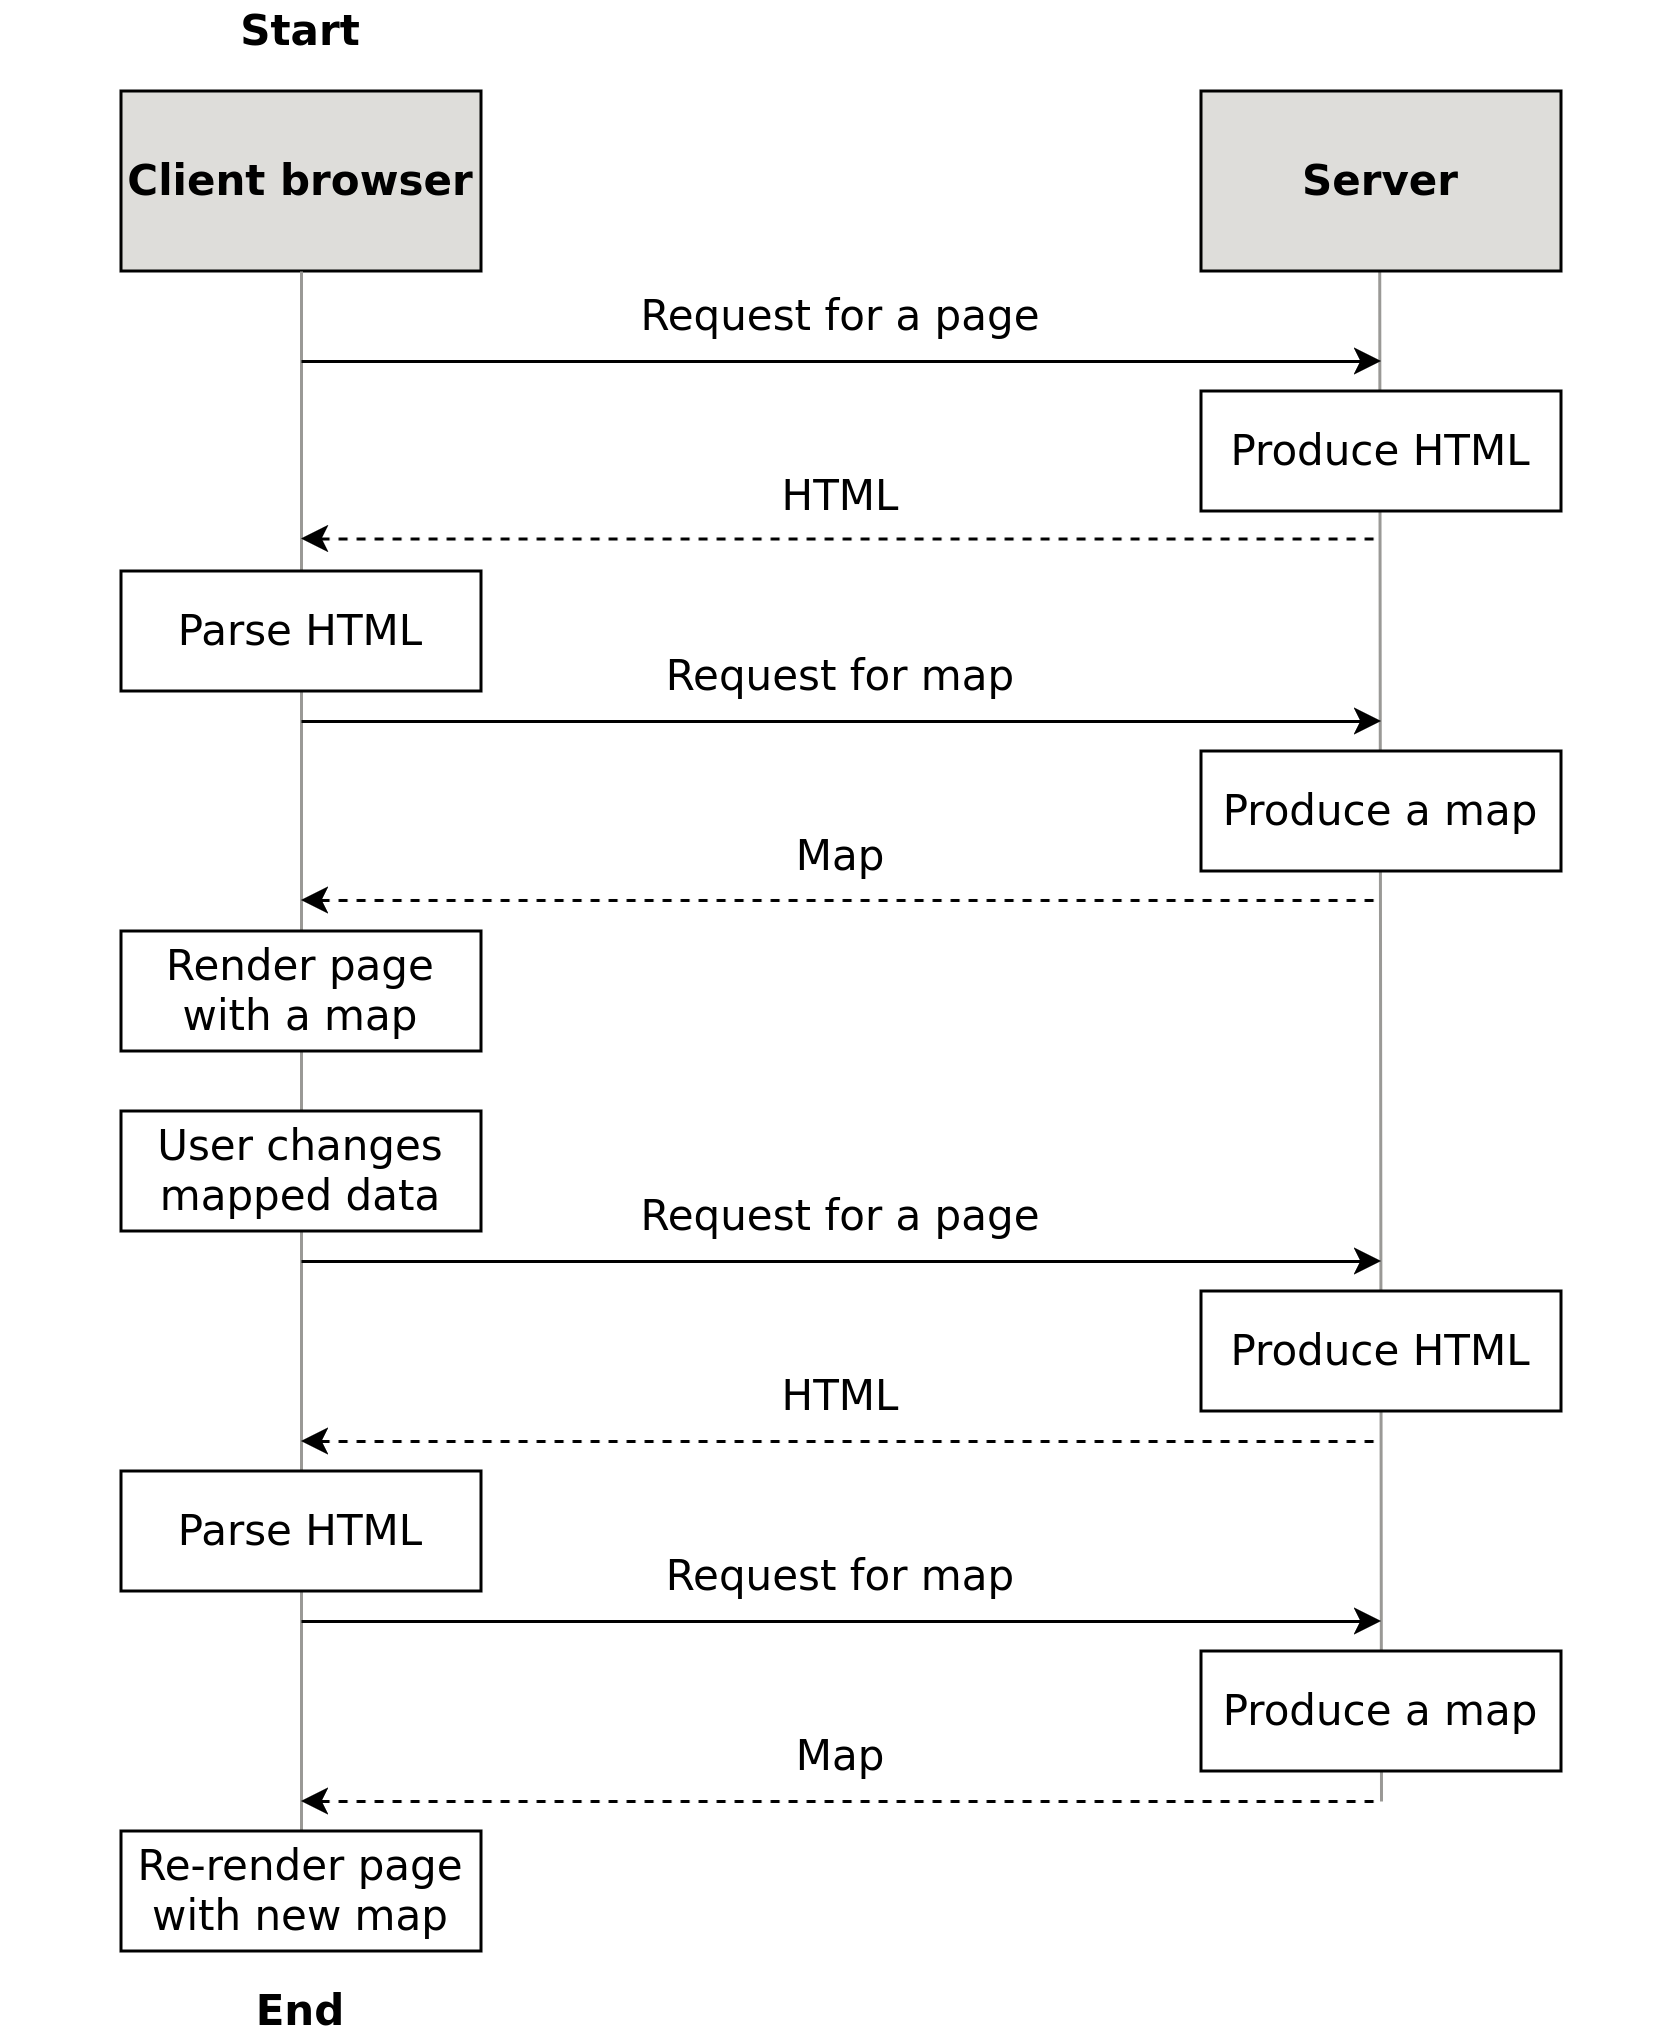
\includegraphics[width=\diagramwidth]{visual/figures/diagrams/server-side-app.png}
	\caption{
		An interactive map of traditional website design.
		All manipulation of the web page and the map happens on the server-side,
		and each change results in a complete re-fetch and re-render of the page.
	}
	\label{fig:server-side app}
\end{figure}

\begin{figure}[H]
	\centering
	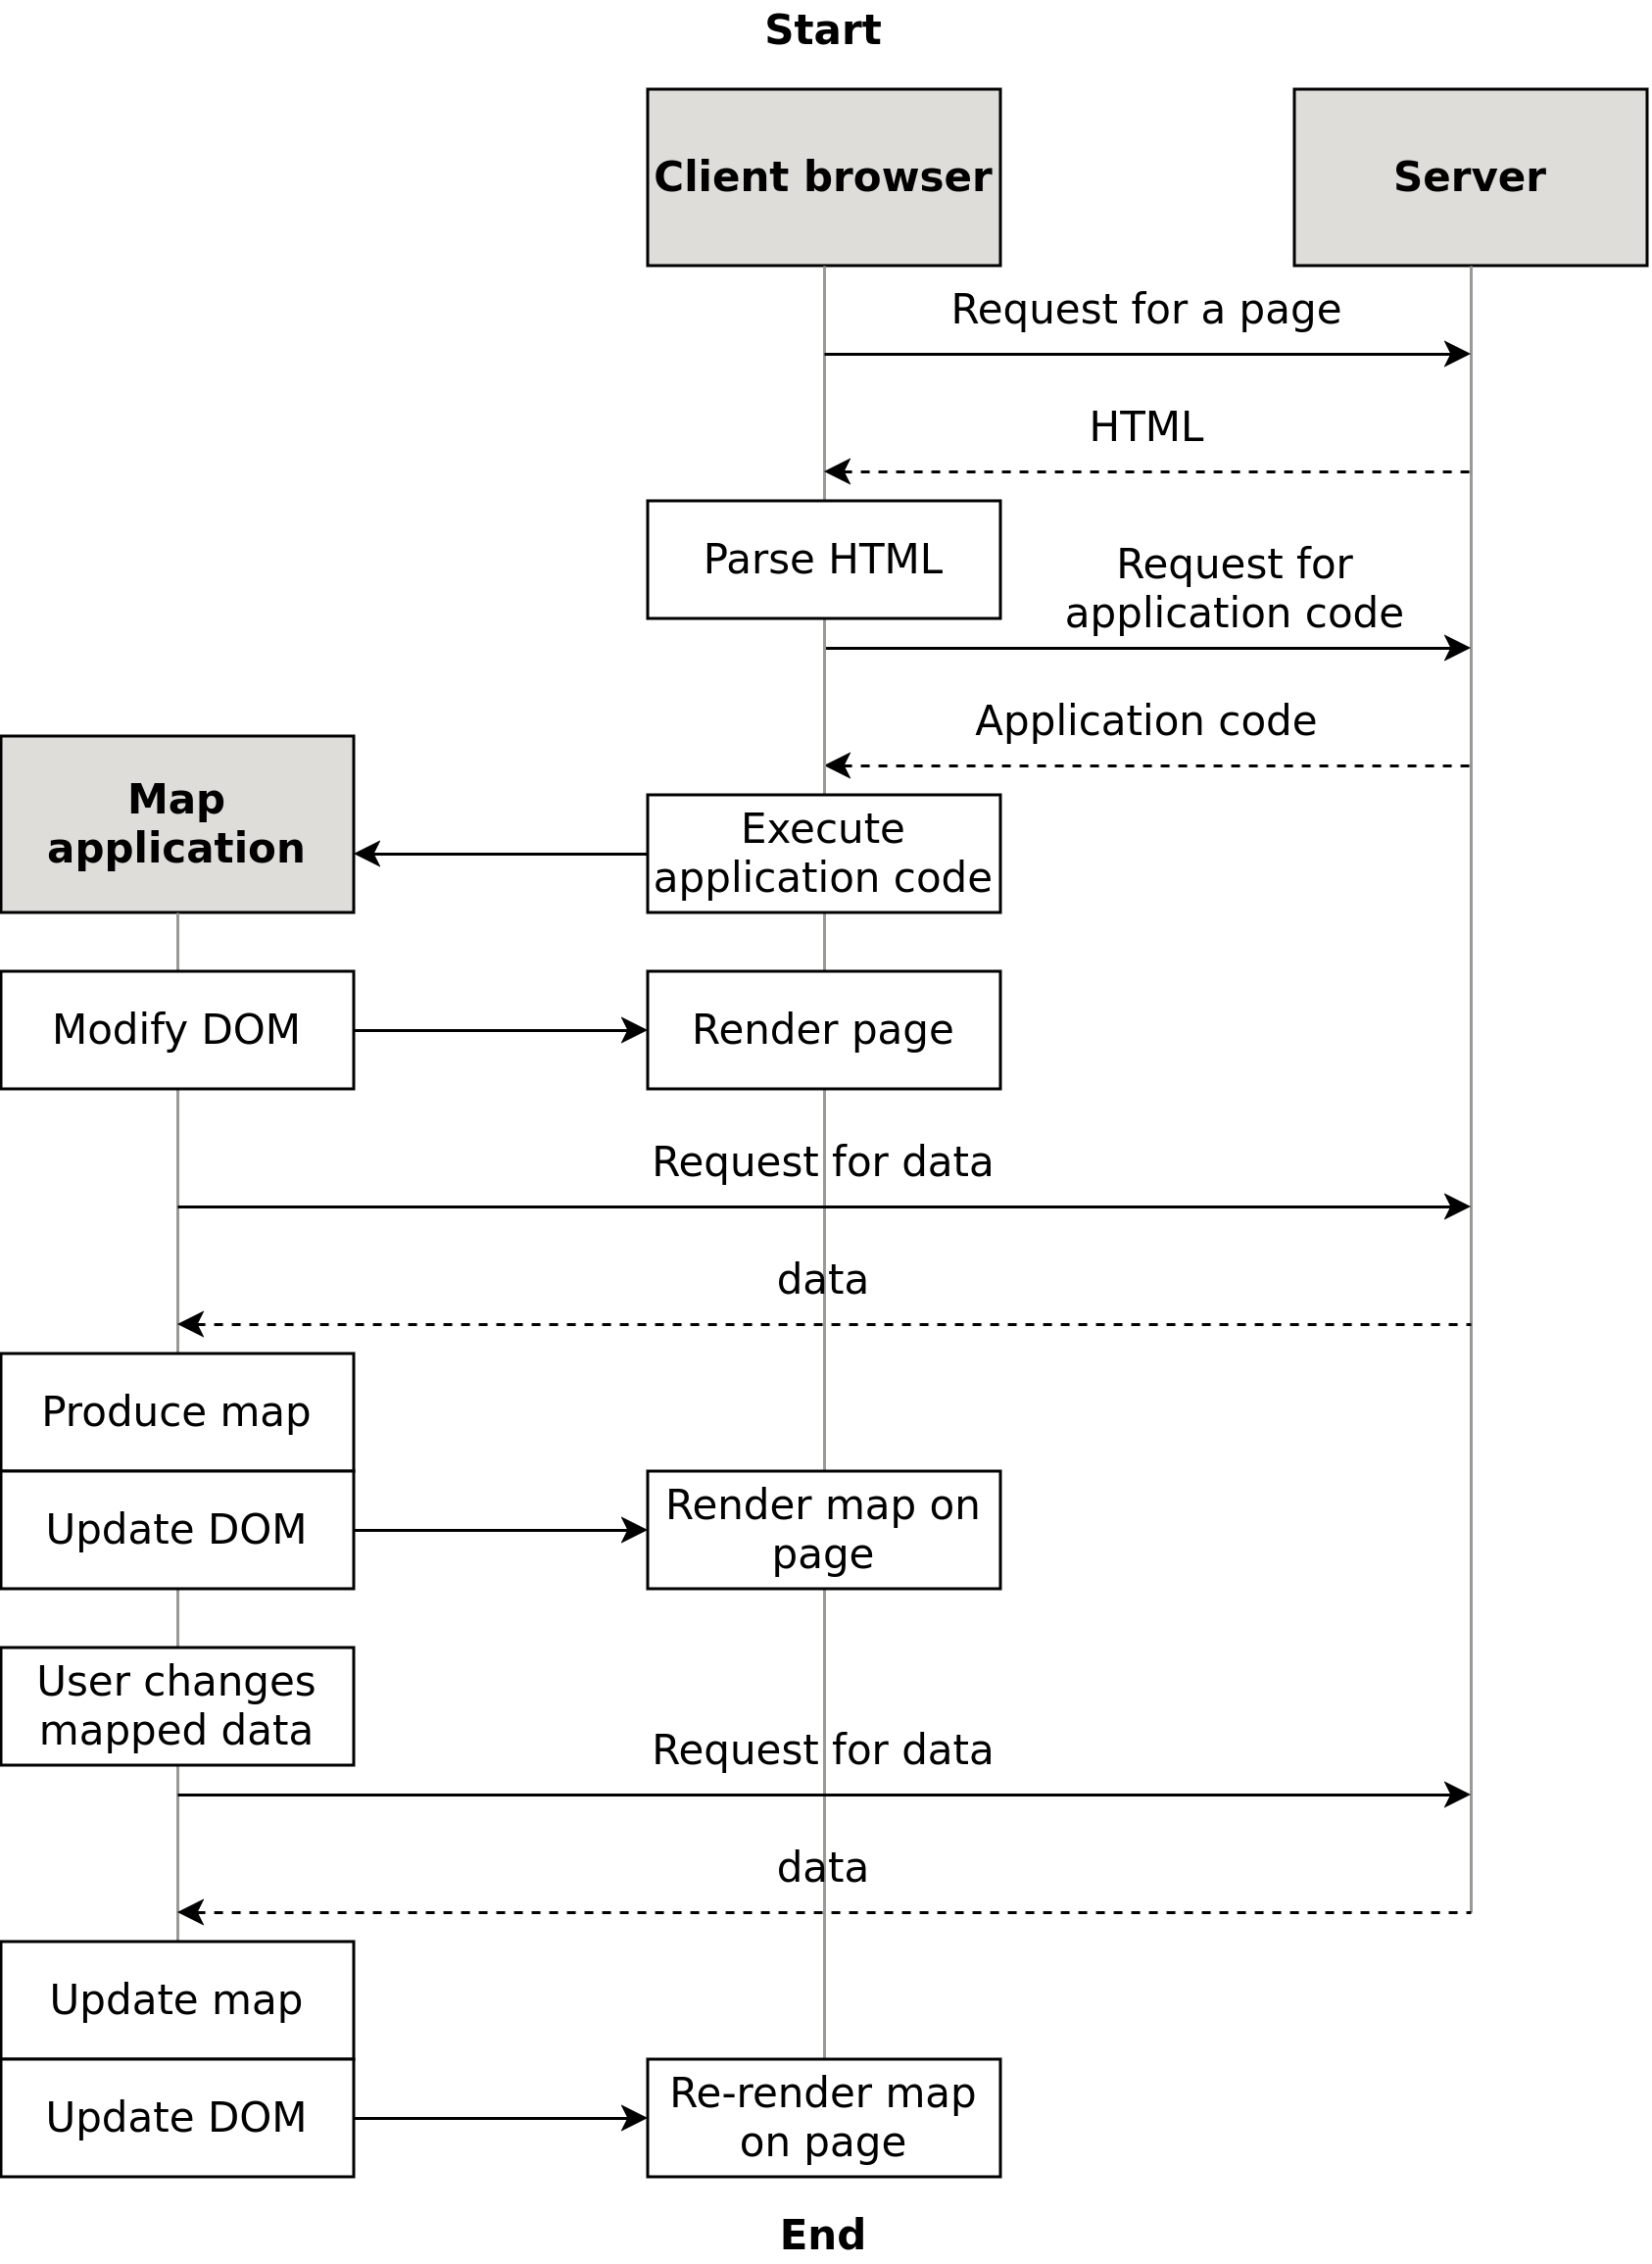
\includegraphics[width=\diagramwidth]{visual/figures/diagrams/spa.png}
	\caption{
		A web map as a \acrshort{spa}. Here the initial page load is more complex,
		but, once the application is running on the client,
		subsequent interactions with the map are handled on the client side.
		Instead of fetching entire new pages from the server,
		updating the map content requires only fetching the necessary data.
	}
	\label{fig:spa}
\end{figure}

As shown above, a \acrshort{spa}-style web map handles mapping,
web page layout and content, and other possible \acrshort{ui} logic
on the client browser.
Also, a \acrshort{spa} manages most, if not all,
application \textit{state} --
in other words, it records, updates and acts on dynamic information about
the condition of the application and its components.
In the system described above \parenfig{spa},
the mapped data could be an example of such state.
The server-side, in comparison,
is essentially stateless and contains no business logic.
The main point here is that the client-side of a
web map system that employs a \acrshort{spa} design
is potentially a very complex piece of software.
Implementing all the functionalities needed for such an application
from the ground up would be an enormous task.
\textit{Software libraries},
in other words external modules of reusable code,
are essential in overcoming this.
From the perspective of web mapping, two types of libraries are especially important.
A \textit{web mapping library} usually provides capabilities for the most common tasks
that a web map is expected to perform:
for example zooming and panning, rendering data on the map,
and downloading and rendering base maps.
Especially if an application gets more complex,
a general purpose \textit{\acrshort{ui} library},
often called a \textit{framework},
can be beneficial in constructing and managing
the general, non-map, \acrshort{ui} components of the application
as well as the application and component state.

This section introduced the necessities for
understanding and crafting interactive maps at a technological level,
with emphasis on web maps and client-side technologies.
Key web mapping concepts are assembled to table \ref{tab:web tech}.
Due to the great breadth of technologies,
the listing is by no means exhaustive --
it includes only the concepts indispensable for cartographic interaction on the web.
 
\begin{table}[H]
	\caption{
		Web tech
	}
	\label{tab:web tech}
	\centering
	\begin{tabular}{ | L{0.15\textwidth} | L{0.75\textwidth} | }
		\hline
		\textbf{Concept / technology}
		& \textbf{Description} \\
		\hline
		\hline
		\acrshort{html}
		& A markup language for describing the content and structure of a web page \\
		\hline
		\acrshort{http}
		& Protocols for transferring information over the internet \\
		\hline
		Client
		& Software that sends requests and receives information, possibly performing computation \\
		\hline
		Server
		& Software that receives requests and responds to them by sending information \\
		\hline
		JavaScript
		& A scripting language for implementing client-side web applications \\
		\hline
		\acrshort{dom}
		& Semantic description of a web page \&
		an \acrshort{api} enabling software to manipulate it \\
		\hline
		\acrshort{ajax}
		& A set of technologies enabling asynchronous client-side software \\
		\hline
		Web mapping library
		& A collection of reusable code with capabilities for typical mapping-related tasks \\
		\hline
		\acrshort{ui} framework
		& A collection of reusable code with capabilities for
		crafting and managing general-purpose \acrshort{ui} components \\
		\hline
	\end{tabular}
\end{table}


% Relevance of web as a platform,
% why web-based applications are the norm
% (in general and, for much of the same reasons, in the context of maps).

% Web technologies and standa:
% % Hypertext Markup
% % Language (HTML) for structuring web content, Cascading Style Sheets (CSS) for styling web content, the Document
% % Object Model (DOM) and the JavaScript scripting language for storing and manipulating web content in browser,
% % JavaScript Object Notation (JSON) for exchanging data in-browser, and Scalable Vector Graphics (SVG) for rendering
% % visual web content, among others (see Sack 2017 for a review)rds,
% define web map  % A web map is a map made with the web standards

% The relevant terms and software architechture (in web context):
% At least the concepts of front / backend and server requests / responses
% are pretty essential to understanding anything about the technical side.

% The relevant technologies, the tools with which interactive maps are made:
% web mapping and user interface libraries, backend solutions
% (not every technology but a concise overview)


% \subsubsection{The process}


\subsection{Cartographic presentation of accessibility}

While in the context of cartography accessibility can be understood as
the ease of reading and using maps,
I use the term here to refer to spatial accessibility.
In general, this type of accessibility can be thought of as a measure of
how easy it is to reach valued destinations in physical space \parencite{lev2020}.
Conceptualizing accessibility
in a holistic manner is not simple.
% geu2004 different measures

While a common starting point for defining the term is, quite concisely,
\enquote{potential of opportunities for interaction} \parencite{han1959},  % define interaction in more detail?
more precise definitions and measurements can be constructed in countless ways
depending on the factors deemed impactful to that potential
\parencite{pap2016}.
For example, even with a simple consideration of travel distance as a measure of access,
including all the different things this access can be measured in relation to
would make the amount of variations, i.e. different \enquote{accessibilities},
to measure grow exponentially \parencite{lev2020}.
In addition, accessibility is inherently tied not only to location
but also time \parencite{jar2018},
meaning every place in every time has a level of access
in relation to every other place.

Because of its composite and dynamic nature,
constructing representative cartographic visualizations of accessibility is difficult.
Accessibility visualizations are often constrained
to displaying access in relation to
a limited number of pre-selected places (for example \textcite{wei2018}),
or composing an accessibility index
that can be calculated and mapped for all locations,
in relation to potentially many different things and locations
(for example \textcite{kim2019}).
However, more complex accessibility measures tend to lead to
less usable presentations \parencite{te2014},
while mapping more simple measures could lead to an influx of variations to present.
For example, separating different travel modes, times of day or target locations
would multiply the amount of visualizations needed to present accessibility.

Even if visualizing every aspect of accessibility
from everywhere to everywhere is impossible,
careful consideration and implementation
of the cartographic methods we have at our disposal might get us closer.
Interactive cartography could be one approach with great potential.
After all, a key principle of interactivity in map presentations is
the map user's ability to change the content of the map \parencite{rot2013b}.
For visualizing accessibility this could mean, for example,
interactive selection of location or travel mode instead of
a static accessibility index that, to a varying extent,
tries to account for everything.
Scientific literature on the topic seems to support the idea of
interactivity in accessibility visualization,
even indicating a need for such presentations.
In a study focusing on the usability of
different accessibility instruments and visualizations,  % accessibility instrument
\textcite{te2014} highlight the importance of
real-time interactivity between the map and the map user.
\textcite{but2018} state that for maps to efficiently communicate accessibility,
they should be as flexible and dynamic as possible.
However, \textcite{but2018} also note that
these qualities are often missing in accessibility visualizations.
Along the same lines,
\textcite{paj2021} find modern accessibility visualizations often complicated,
and lacking in interactivity and flexibility.

Different conceptualizations of accessibility,
their implications in presenting the phenomenon.

In general: people, transport, activities make up accessibility.
A multi-location, multimodal, multi-temporal phenomenon.

Approaches in visualizing accessibility:
Examples of static and interactive accessibility maps.
Simple measures vs complex measures,
High interactivity vs low interactivity.

Isochrones as an example of a simple measure / visualization approach:

\begin{figure}[H]
	\centering
	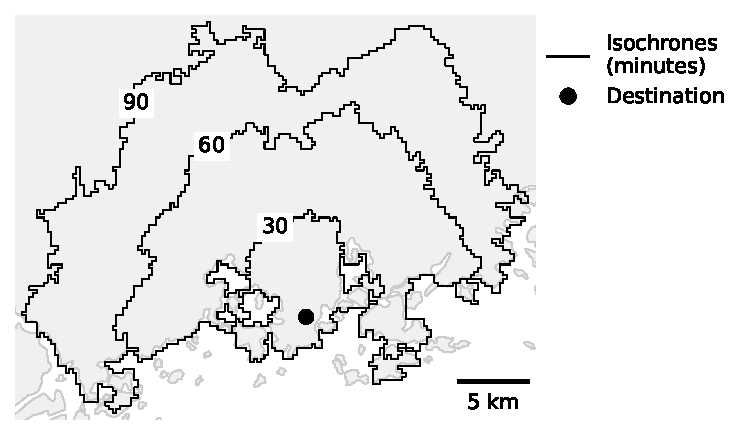
\includegraphics[width=0.6\textwidth]{visual/figures/ttm/isochrone_lines.pdf}
	\caption{Isochrones}
	\label{fig:isochrone lines}
\end{figure}

\begin{figure}[H]
	\centering
	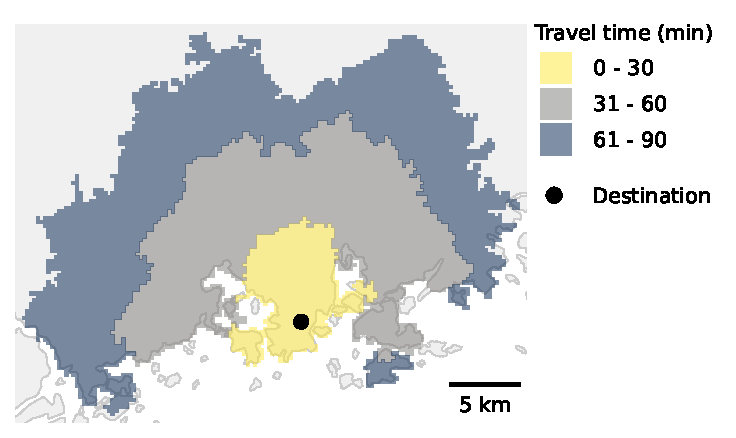
\includegraphics[width=0.6\textwidth]{visual/figures/ttm/isochrone_areas.pdf}
	\caption{Areas between isochrones}
	\label{fig:isochrone areas}
\end{figure}

SIDENOTE: How should I refer to isochrones when I mean the polygons instead of lines?

% TODO
% Mention tradeoffs (detail - speed) -> leads to methods
% Crafting any cartographic presentation is much about tradeoffs.
% Often these tradeoffs are concerned with the visual composition of the presentation --
% what the map can and should try to communicate.

% TODO
% Previous presentations can be very precise, but locked to a single place

